\documentclass[oneside,a4paper,11pt,explicit]{book}
\usepackage[utf8]{inputenc}
\usepackage{icecream}
\usepackage[english]{babel}
\addto\captionsenglish{\renewcommand{\chaptername}{}}
\usepackage[accsupp]{axessibility}  % improves PDF readability for those with disabilities.
\usepackage[colorlinks = true,urlcolor  = blue,linkcolor = blue]{hyperref}
\usepackage{setspace}
\usepackage{listings}
\usepackage[most]{tcolorbox}
\usepackage{minitoc}


\renewcommand{\mtifont}{\large\sffamily}
\renewcommand{\mtcfont}{\small\sffamily}
\renewcommand{\mtcSfont}{\small\sffamily}
\renewcommand{\mtcSSfont}{\small\sffamily}
\renewcommand{\mtcSSSfont}{\small\sffamily}
\mtcsetpagenumbers{minitoc}{off} % turn off page numbering in minitocs
\addto{\captionsenglish}{% Making babel aware of special titles
	\renewcommand{\mtctitle}{Quick Links To Sections}
}
\setlength{\fboxrule}{5pt}
\setlength{\fboxsep}{4pt}

\definecolor{IceCreamLeaf}{rgb}{0.4, 0.639215686274, 0.4}
\definecolor{IceCreamOrbit}{rgb}{0.803921568627451, 0.3607843137254902, 0.3607843137254902}

\pretolerance=10000
\tolerance=2000 
\emergencystretch=10pt

%%%%%%%%%%%%%%% END PREAMBLE

\title{I.C.E.C.R.E.A.M. Tutorials}
\subtitle{\small Observing Earth from Above (Env 329) - Fall 2023  \\
	\small Schmid College of Science and Technology, Chapman University}
\date{\today}

%% DOCUMENT
\setstretch{1.25}
\makeatletter
\begin{document}
	
	\dominitoc
	
	%\tableofcontents
	
	\setcounter{chapter}{3} %Insert (Tutorial Number-1) Here; example for tutorial 4, enter 3
	
	\chapter{Hometown Temperature Competition} %Enter Tutorial Name Here
	
	\vspace{-2em}
	
	\minitoc
	
	\hrule
	
	\vspace{1em}
	
	\begin{tcolorbox}[enhanced,frame style image=blueshade.png,
		opacityback=0.75,opacitybacktitle=0.25,
		colback=blue!5!white,colframe=blue!75!black,title={\Large \textbf{Objectives:}}]
		\large
		\begin{enumerate}
			\item Create your own shapefiles in QGIS. 
			\item Learn about cloud filtering options in A$\rho\rho$EEARS.
			\item Access and download land surface data from ECOSTRESS of the highest and lowest temperatures in 2022 for your hometown, favorite place you have lived, or somewhere you wish to move in the future.
		\end{enumerate}
	\end{tcolorbox}
	
	\clearpage
	
	%%%%%%%%%%%%%%%%%%%%%%%%%%%%%%%%%% Change Header to Have a Smaller Logo for Remainder of the Document
	\fancyhead{}
	\fancyhead[C]{\begin{tikzpicture}[overlay, remember picture]
			\fill[Blue2] (current page.north west) rectangle ($(current page.north east)+(0,-1in)$);
			\node[anchor=north west, text=white, font=\Large, minimum size=1in, inner xsep=5mm, align=left] at (current page.north west) {\bf{\MakeUppercase{\@title}}\\\@subtitle};
			\node[anchor=north east, minimum size=1in, inner xsep=5mm] at (current page.north east) {\includegraphics[scale=.125]{ICECREAM_Logo.png}};\end{tikzpicture}}
	%%%%%%%%%%%%%%%%%%%%%%%%%%%%%%%%%%
	
	\noindent\fbox{\begin{minipage}{.9665\textwidth}
			
			\vspace{1em}
			\begin{center}
				\textbf{\Large \underline{Motivation For Today's Tutorial : Temperature Competition}}
			\end{center}
			
			\vspace{1 em}
			
			\centerline{
\includegraphics[width=.75\textwidth]{Hometown.png}}
			
			\vspace{1 em}
			
			
			For this tutorial, we are going to combine the skills you have learned so far and enter you into a little competition to see who had the hottest and coldest hometown temperatures for 2022. You are welcome to use your hometown, favorite place you have lived, or somewhere you wish to move in the future. 
			
	\end{minipage}}
	
	\vspace{1 em}

	\section{Hometown Temperature Competition Progress}

In the last tutorial (\href{https://jeremydforsythe.github.io/icecream-tutorials/Tutorial4_TemperatureCompetition/Tutorial4_TemperatureCompetition.pdf}{Tutorial \#4: Hometown Temperature Competition}) you learned how to draw a shapefile. Your assignment before today's tutorial was to create a shapefile of your hometown, favorite place you have lived, or somewhere you wish to move in the future and use that file in A$\rho\rho$EEARS to download ECOSTRESS land surface temperature data for last year. Then you were to save GeoTIFF files to your computer of the hottest and coldest land surface temperature observations of that year for your hometown.

\begin{tcolorbox}[colback=yellow!5!white,colframe=IceCreamLeaf,title=\textbf{Temperature Competition Next Steps}]
	Now that you have that data let's put it all together in a map.
	\begin{enumerate}
		\item Start a new project and load the shapefile for your hometown, favorite place you have lived, or somewhere you wish to move in the future.
		\item Use the same procedure we followed in this tutorial to create a map with two insets, one for the hottest and coldest days from the last full calendar year using the GeoTIFF files you saved from the previous tutorial. I have included an example on the next page that I made for Vancouver Island in 2022 for inspiration. You already have all of the skills to make this map! You don't have to make one that exactly mimics the example, but it needs to include all of the design elements that make an effective map: north arrow(s), scalebar(s), title(s), and legend(s). Be creative and curious by exploring the menu options and design a beautiful map that clearly communicates the hottest and coldest temperatures while showcasing your individual style.
	\end{enumerate}
\end{tcolorbox}

\centerline{\includegraphics[width=\textwidth]{Vancouver Island Temperature Competition Example.png}}

	
	\section{Creating a Shapefile in QGIS}
	
	In the previous tutorials, we provided you with a shapefile of Death Valley. Remember that shapefiles are a type of file that stores data on locations, shapes and attributes of geographic features. Today, you are going to learn how to create your own in QGIS. We are also going to introduce you to another plugin that can make working with latitude and longitude data in QGIS easier. Let's install Lat Lon Tools. 
	
	\subsection{Installing the \textit{Lat Lon Tools} Plugin}
	
	1. Open QGIS and start a new project by selecting the \textit{Project} menu $\rightarrow$ then \textit{New}. 
	
	2. To install the Lat Lon Tools plugin, click on the \textit{Plugins} drop down menu and select \textit{Manage and Install Plugins}.
	
	3. In the next window, make sure \textit{All} is selected in the first window pane and search for \textit{Lat Lon Tools}.
	
	4. Click \textit{Install Plugin}, wait for the installation to complete, then close the plugin window.
	
	\centerline{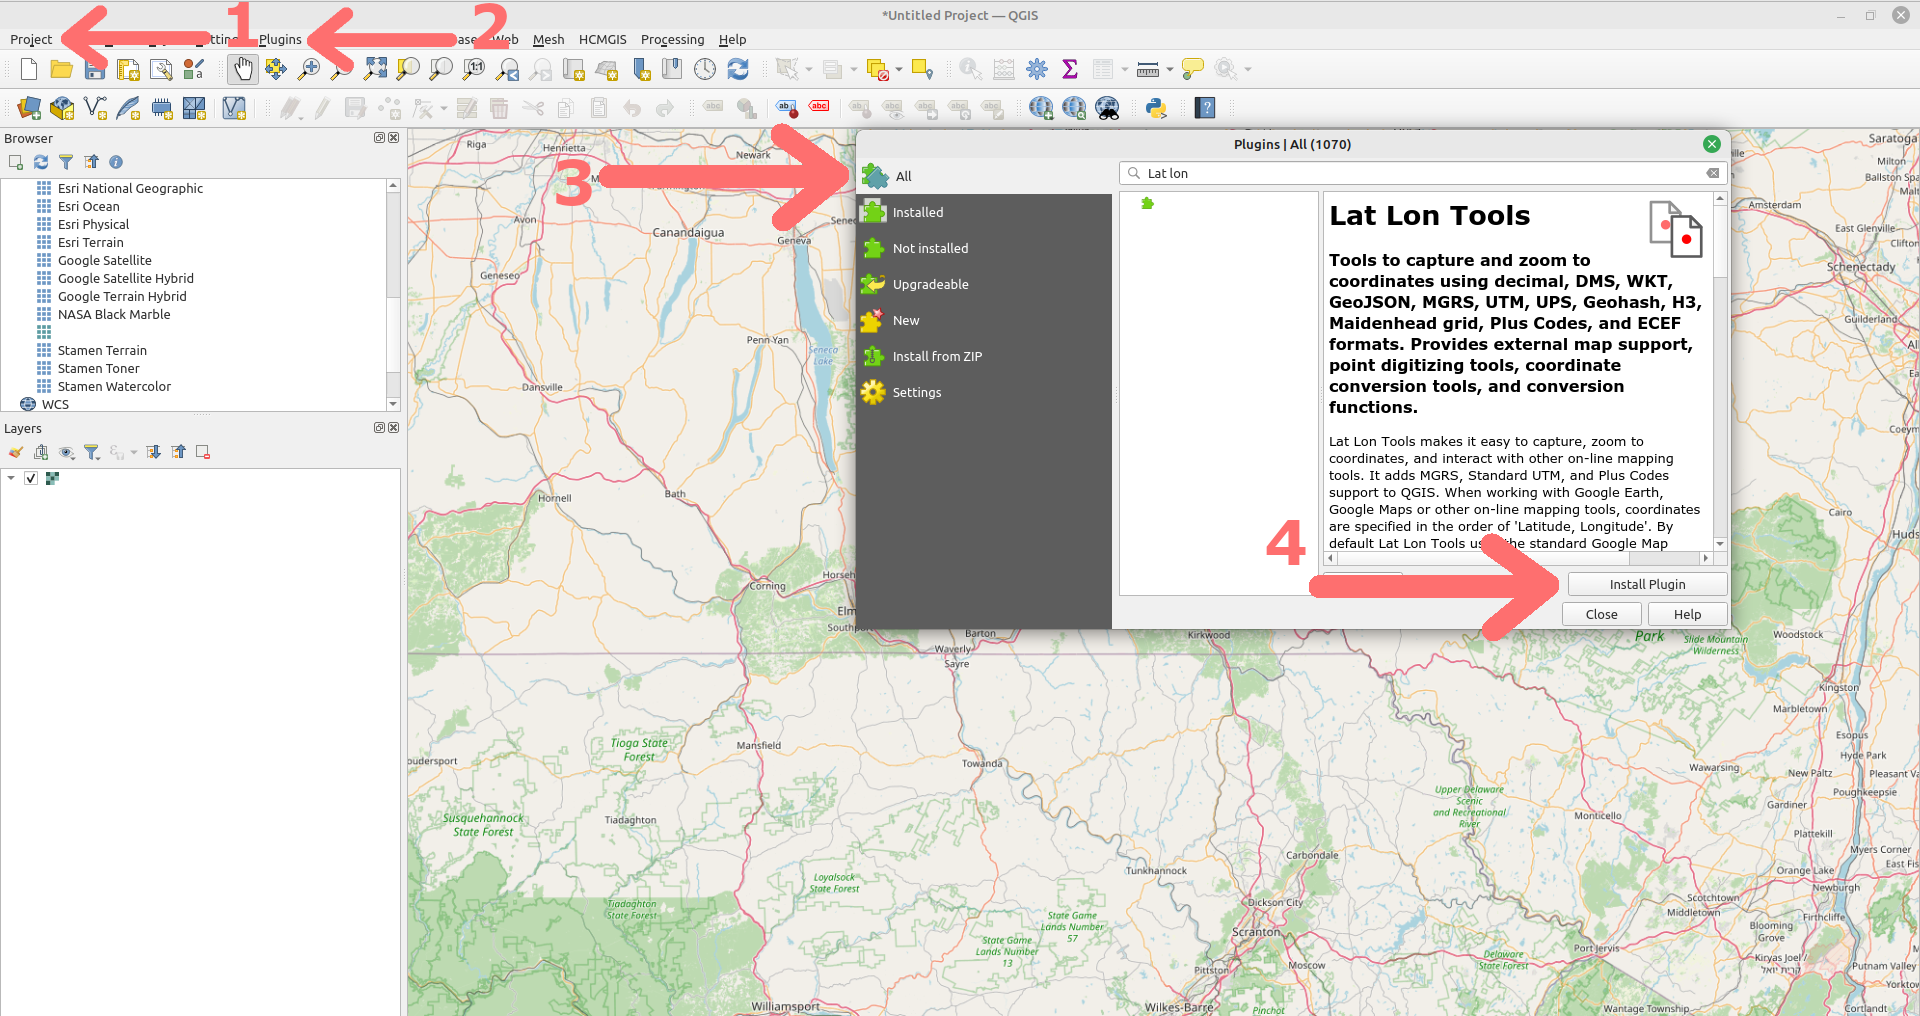
\includegraphics[width=\textwidth]{LatLonTools.png}}
	
	\subsection{Adding an Open Street Basemap Layer}
	
	\centerline{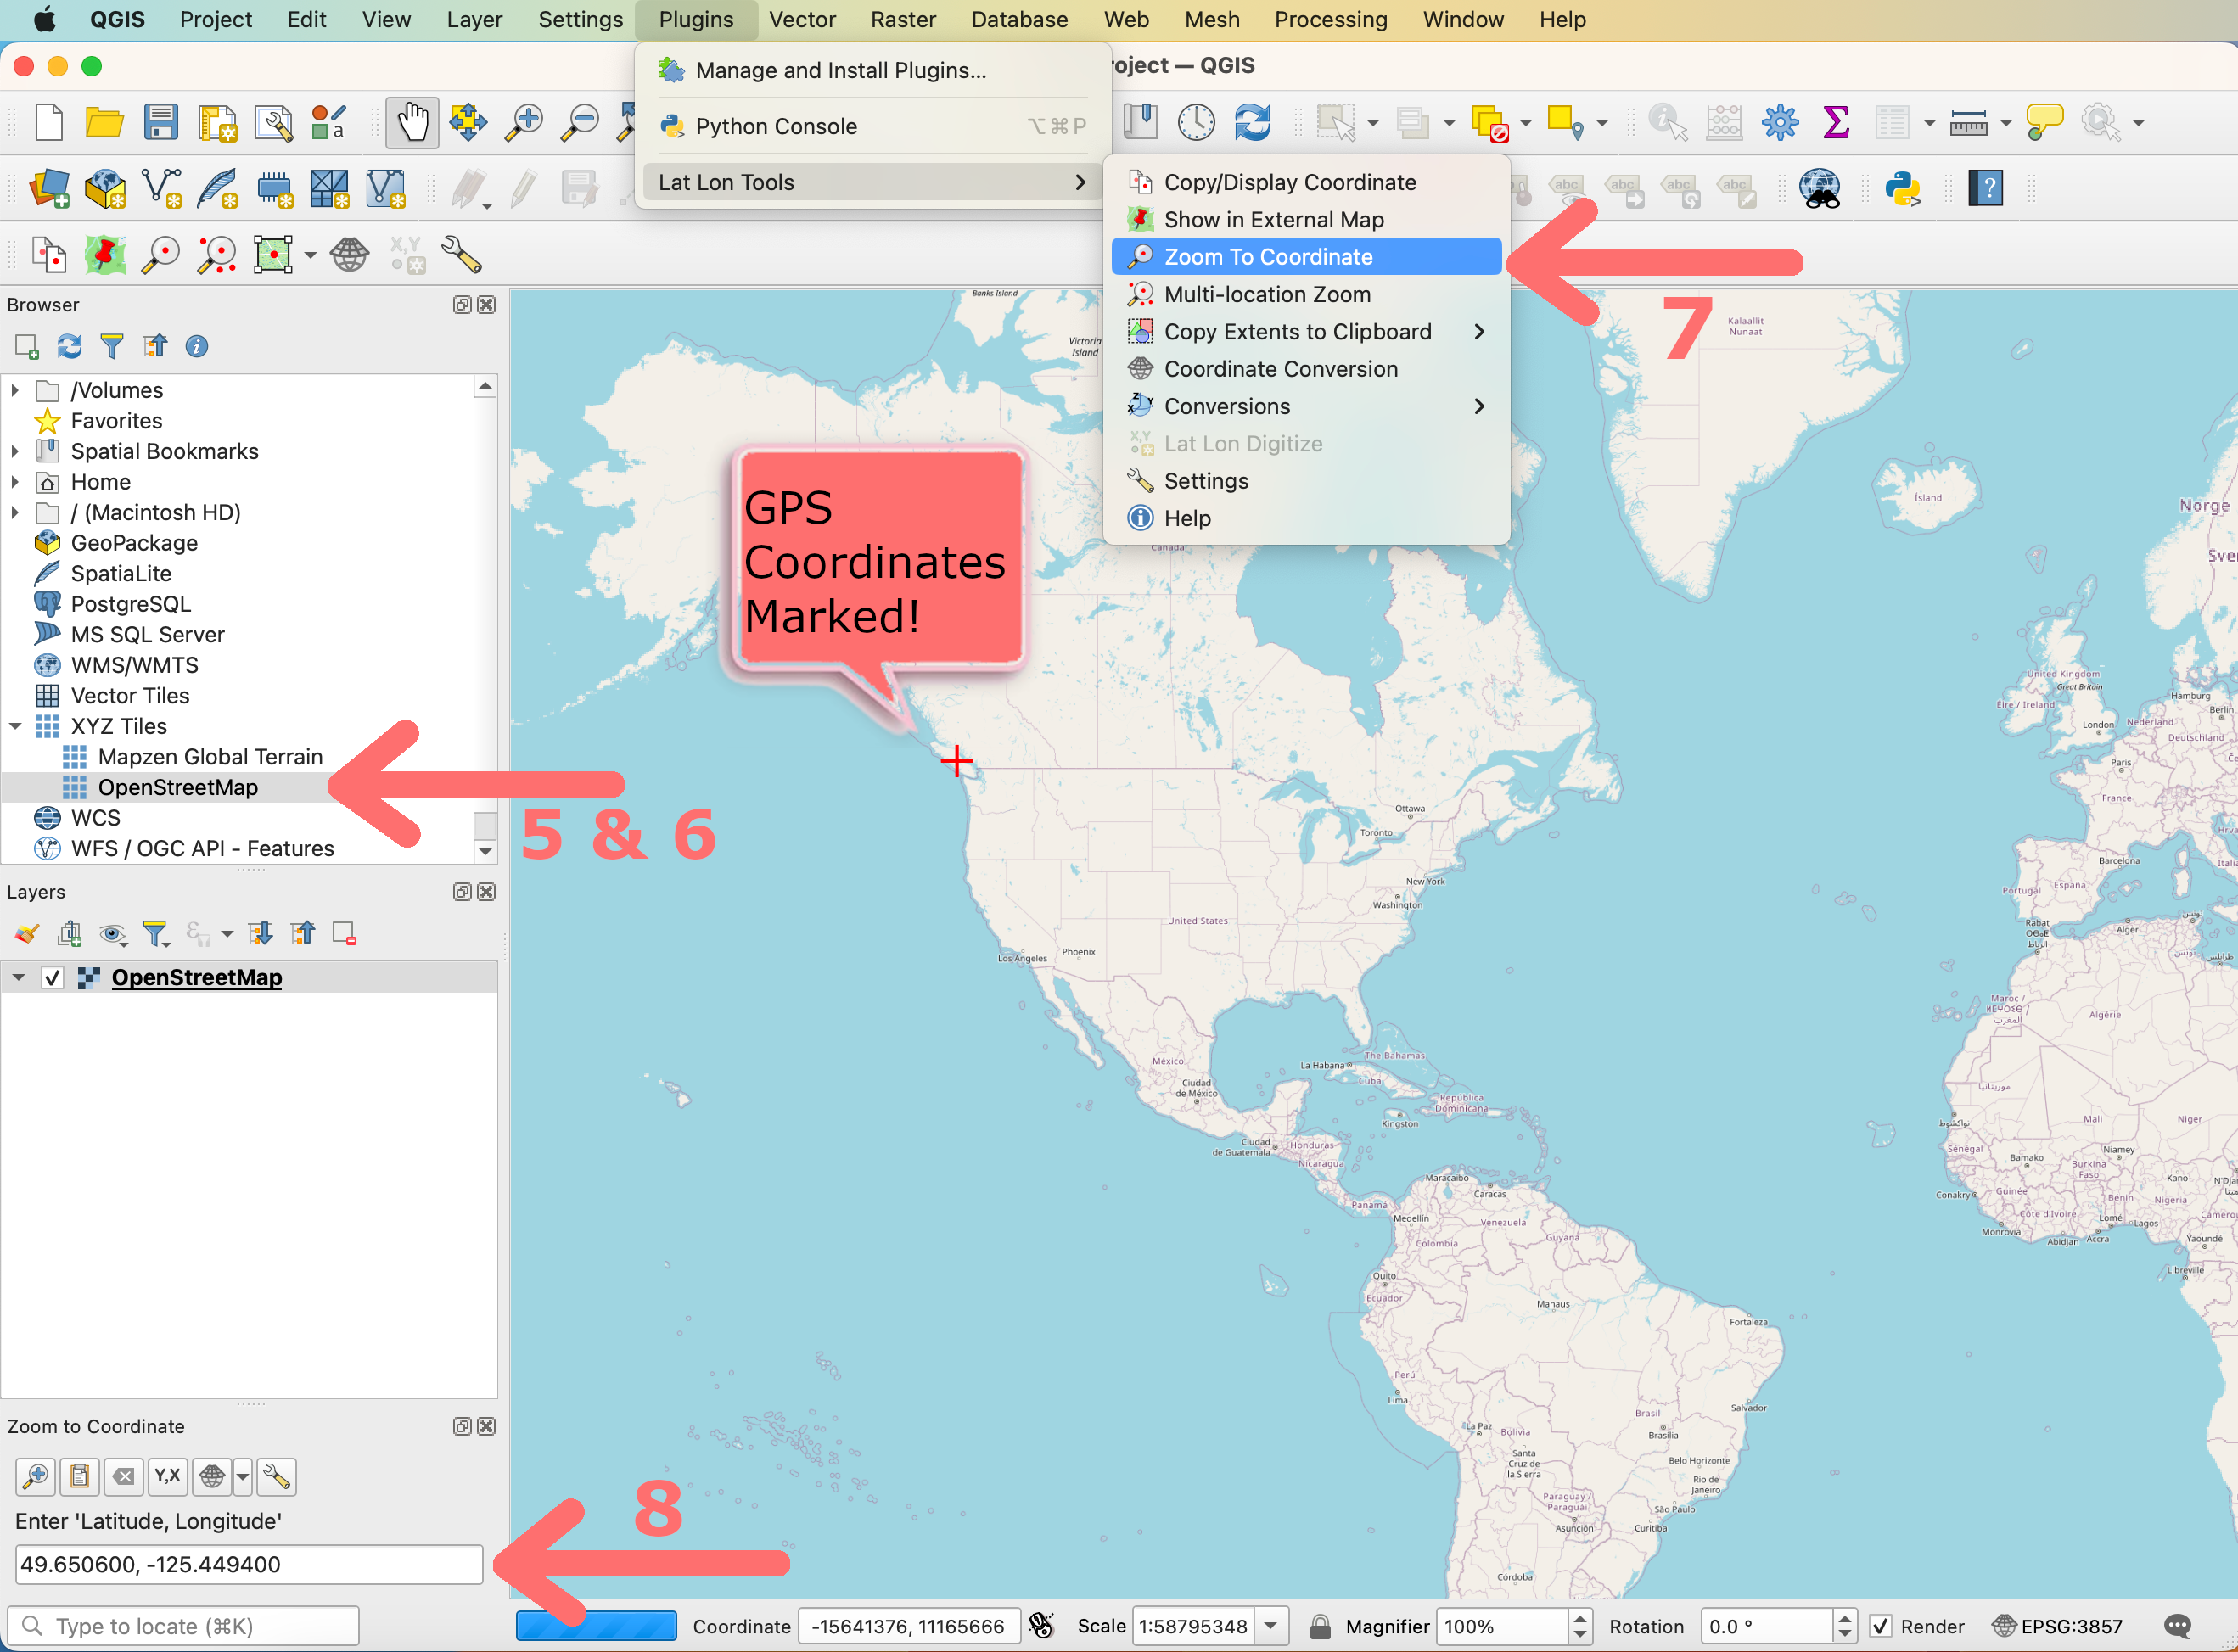
\includegraphics[width=.9\textwidth]{QGISbasemap.png}}
	
	5. In the browser window, expand your options by clicking on the small arrow next to \textit{XYZ Tiles}.
	
	6. Double click on Open Street Map to load in a basic open source map. You will notice that we just added a layer to the layer window below.
	
	\subsection{Finding GPS Coordinates with \textit{Lat Lon Tools}}
	
	Let's say you were interested in requesting and downloading ECOSTRESS land surface temperature (LST) data for Vancouver Island. You need to tell A$\rho\rho$EEARS where Vancouver Island is located, then request and download the data before you can make a map of the results. The first step is to find the island on the basemap we just added.
	
	7. Open up the Lat Lon Tools window by selecting the \textit{Plugins} menu $\rightarrow$ \textit{Lat Lon Tools} $\rightarrow$ \textit{Zoom To Coordinate}.
	
	8. Enter in the following GPS coordinates (formatted as latitude, longitude) : 49.650600, -125.449400. Note that if you are not sure of a location's latitude and longitude, you can navigate to that location in Google Maps and right click on the location to display the coordinates. 
	
	9. The Lat Lon Tools plugin has found the GPS coordinates for Vancouver Island and marked them with a ``$+$'' on the map. 
	
	\subsection{Drawing a Shapefile}
	
	\centerline{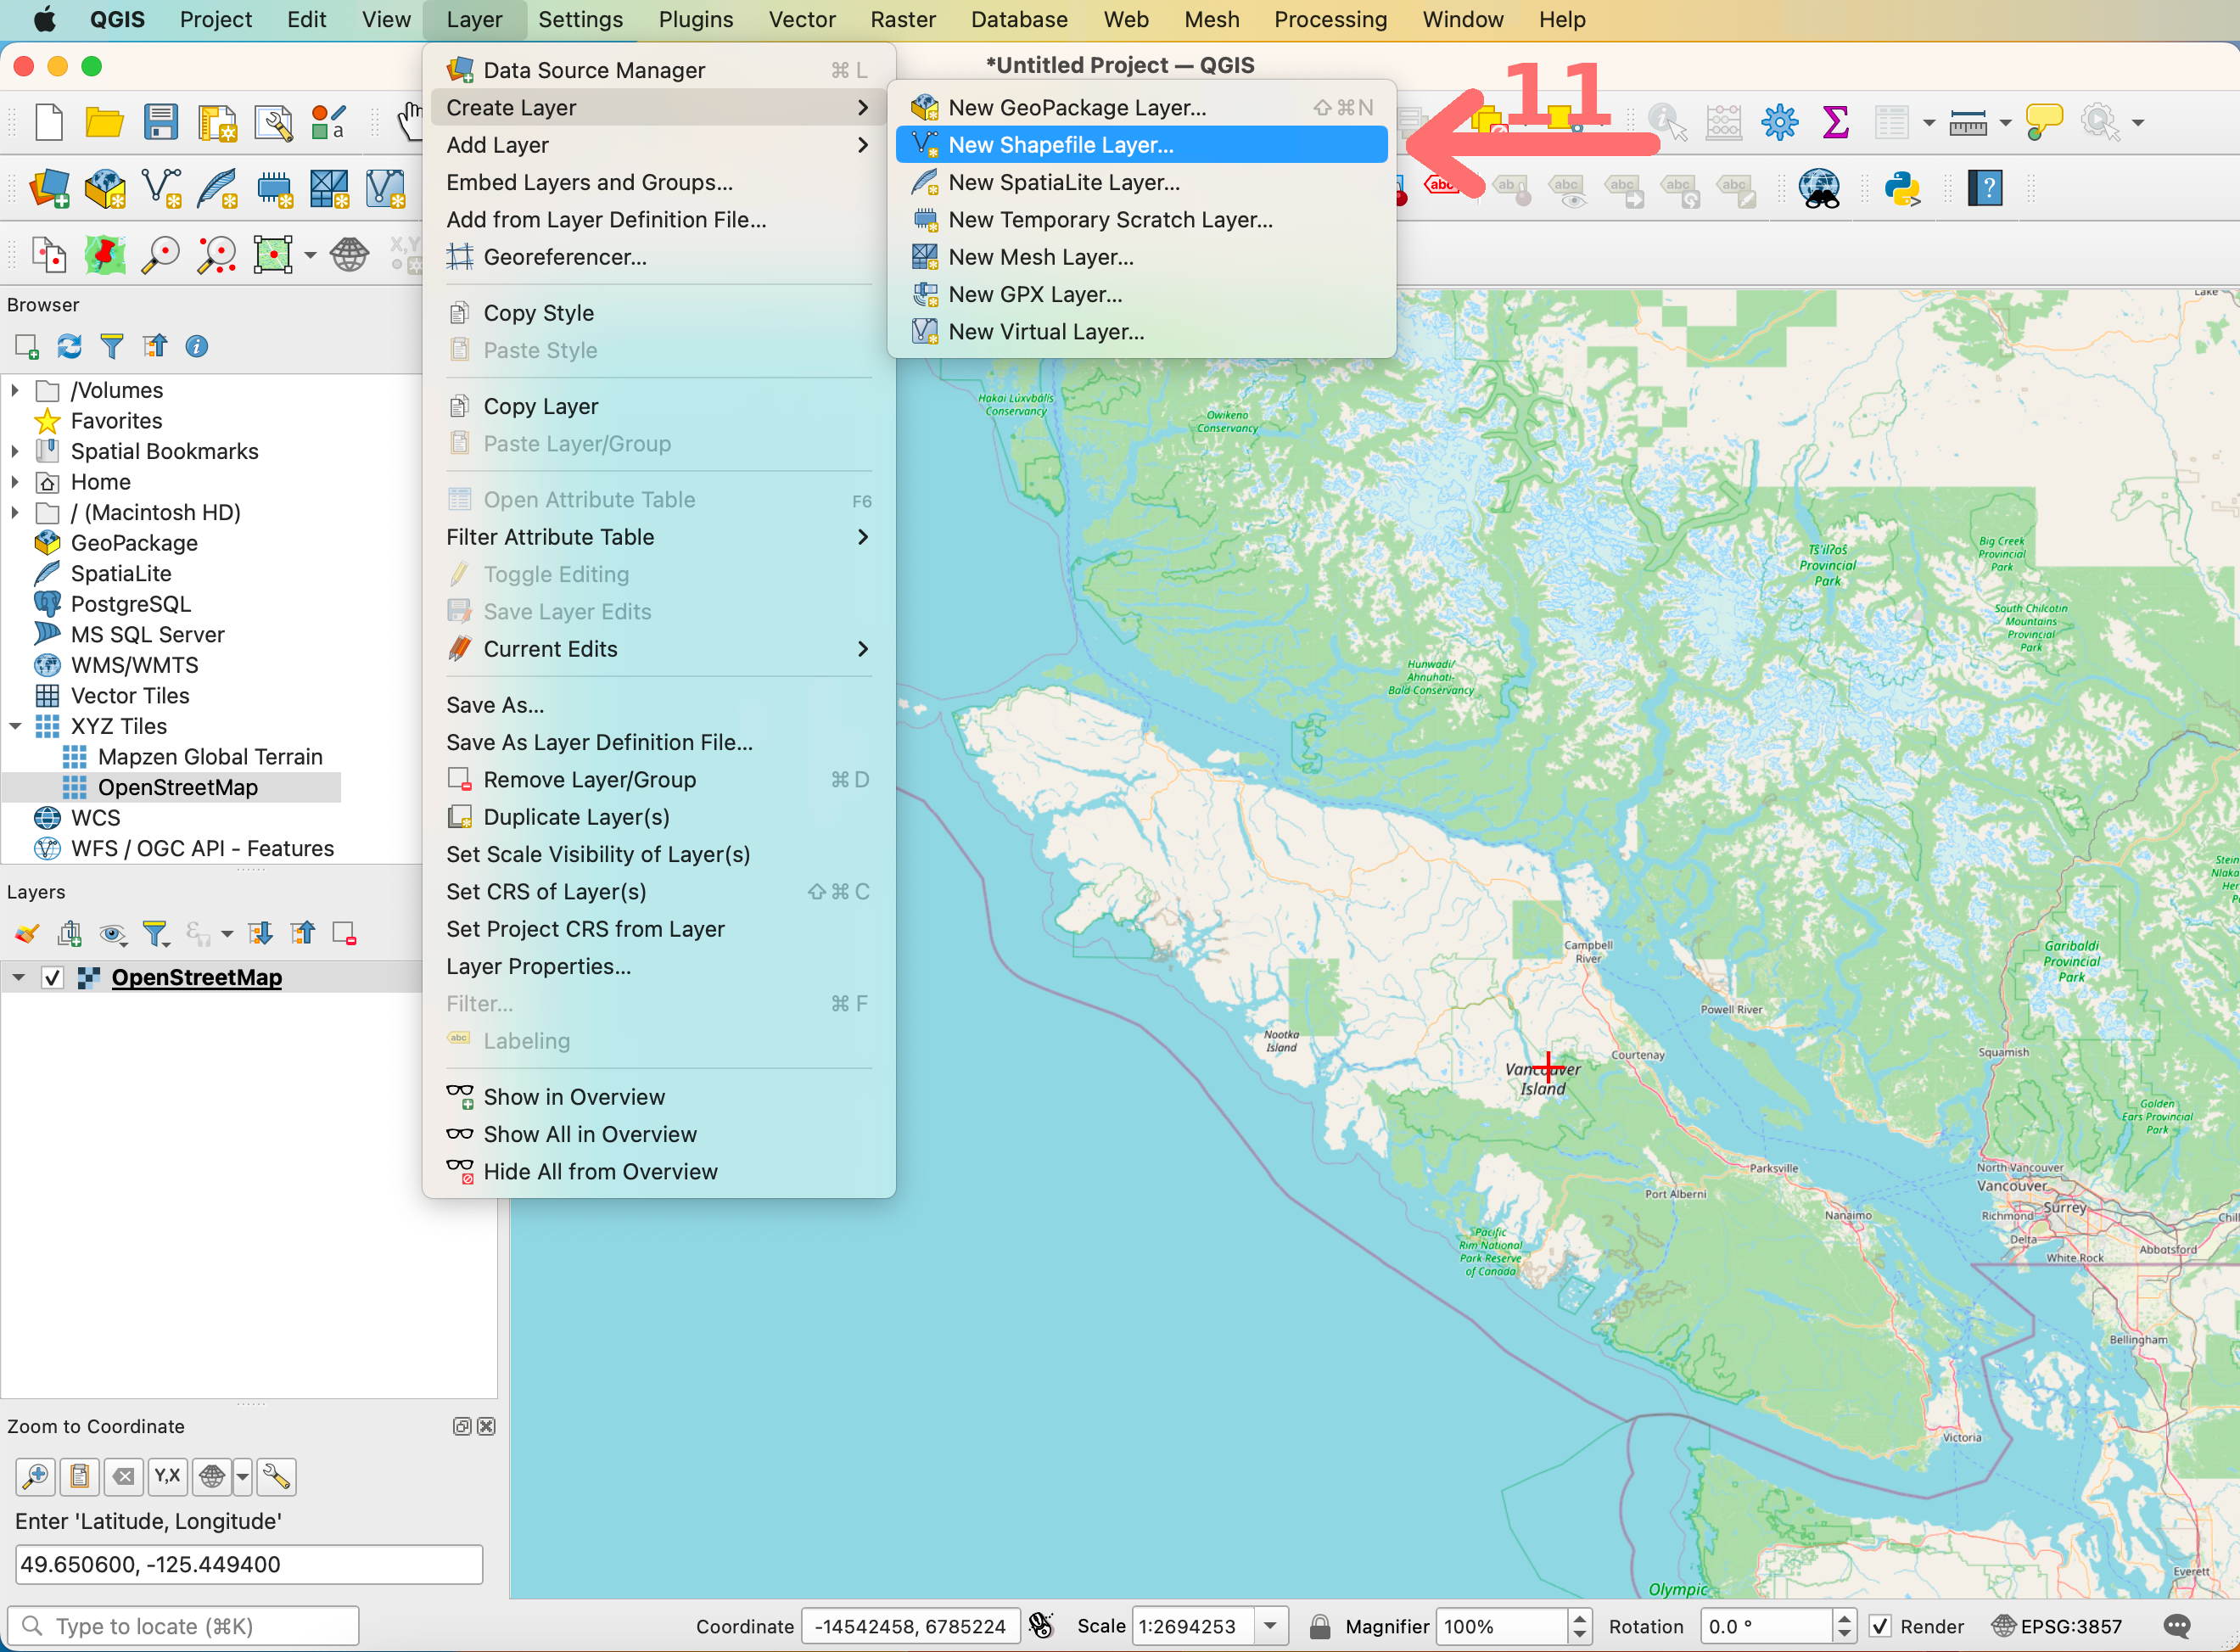
\includegraphics[width=.9\textwidth]{CreateLayer.png}}
	
	Next, we want to draw a polygon (i.e., a line that forms the perimeter of the area of interest) that encompasses Vancouver Island, so that we can pull the request and download the data from A$\rho\rho$EEARS.
	
	10. Zoom in to the GPS coordinates we entered and marked with a ``$+$'' on the basemap using the \textit{zoom in} 
\includegraphics[height=\fontcharht\font`\B]{mActionZoomIn.png}, \textit{zoom out} 
\includegraphics[height=\fontcharht\font`\B]{mActionZoomOut.png}, and \textit{pan} 
\includegraphics[height=\fontcharht\font`\B]{mActionPan.png} buttons in toolbar. If you are on a laptop, you could use the trackpad to do the same.
	
	11. Next, we are going to create a new layer in the map by selecting the following menus: \textit{Layer} $\rightarrow$ \textit{Create Layer} $\rightarrow$ \textit{New Shapefile Layer...}
	
	\centerline{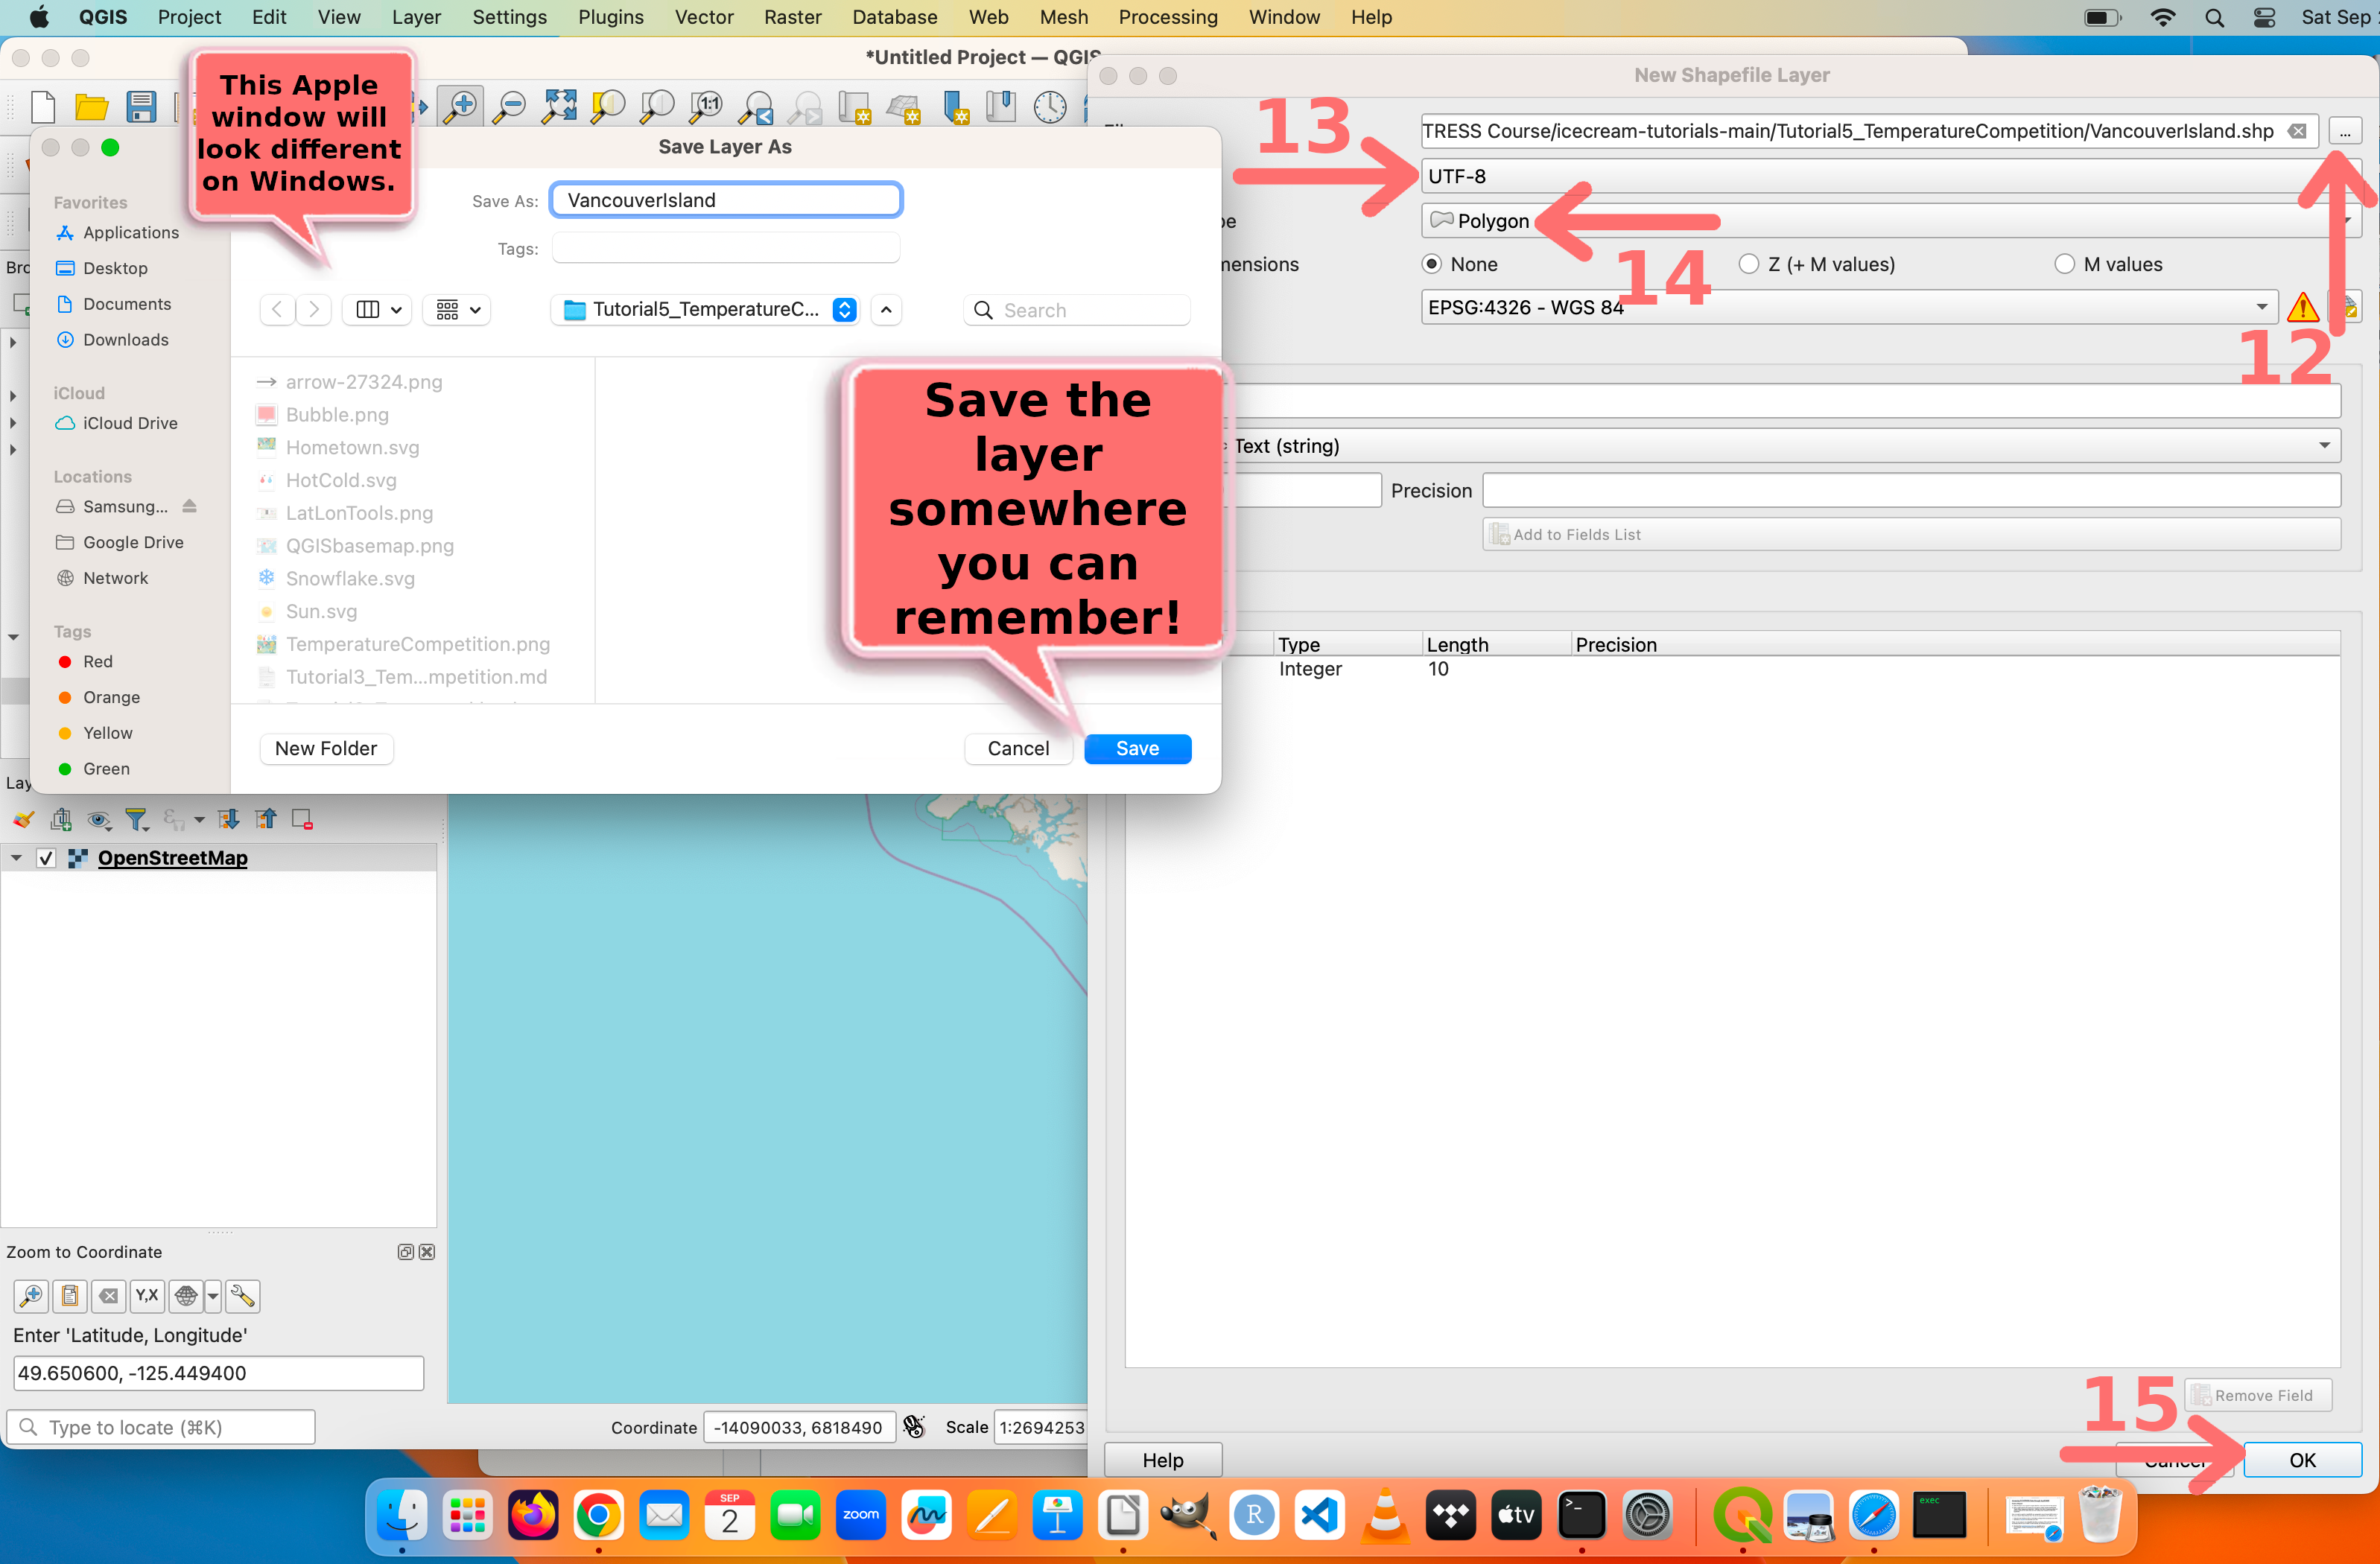
\includegraphics[width=.9\textwidth]{SaveLayer.png}}
	
	12. Select the ``...'' option next to the \textit{Filename} input window. Navigate somewhere you can remember and save it with a worthy filename. ``Vancouver Island Perimeter'' seems appropriate.
	
	13. Select \textit{UTF-8} for \textit{File encoding}.
	
	14. Select \textit{Polygon} for geometry type. 
	
	15. Leave the remaining options as their defaults and click \textit{OK}.
	
	\centerline{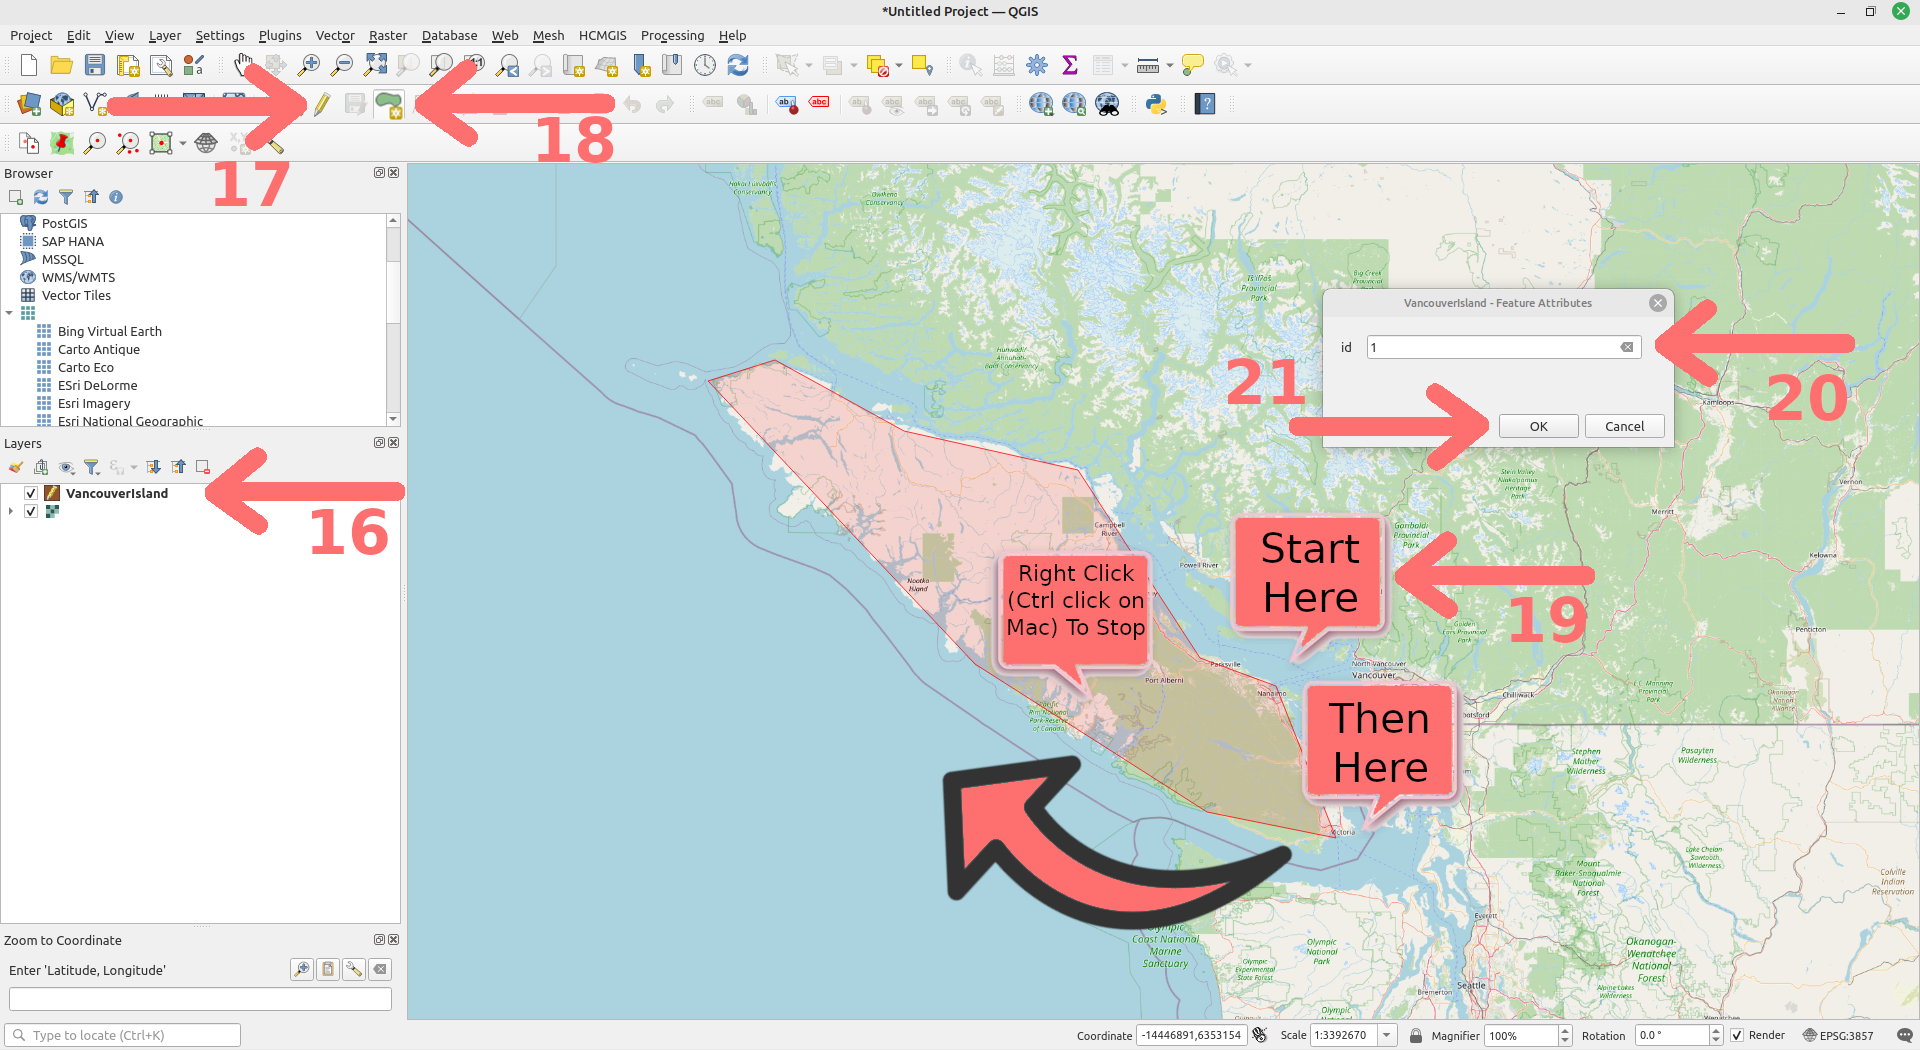
\includegraphics[width=\textwidth]{DrawPolygon.png}}
	
	16. Now, it is time to draw the polygon. First, make sure that your new ``Vancouver Island'' layer is highlighted in the \textit{Layers} window. 
	
	17. Select the \textit{Toggle Editing} 
\includegraphics[height=\fontcharht\font`\B]{mActionToggleEditing.png} button from the toolbar to start editing the layer. 
	
	18. Then select the \textit{Add Polygon Feature} 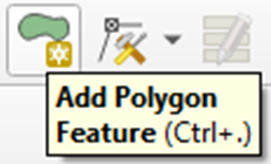
\includegraphics[height=10mm]{addpolygon.png} button to begin drawing your shapefile. 
	
	19. Draw a polygon that encompasses Vancouver Island. Don't worry too much about being perfect, getting the basic shape will do. Right click on Windows or Linux and Ctrl click on Mac to stop drawing when your shape is complete.
	
	\kulbox{\textbf{NOTE:} Drawing a polygon in QGIS is both straightforward and nuanced. You use successive clicks with your mouse to create your desired shape. Simple forms like squares or rectangles are easy achievable, while more complex designs take some practice to master. My recommended route is to start by clicking near Parksville then proceed clockwise around the island. See the screenshot above (step 19).}
	
	20. After you finish drawing, QGIS will prompt you for a feature ID. This is an arbitrary designation for our purposes today, so simply using the number 1 is my recommendation. 
	
	21. Click \textit{OK}. 
	
	22. Select the \textit{Toggle Editing} 
\includegraphics[height=\fontcharht\font`\B]{mActionToggleEditing.png} button from the toolbar to toggle off editing the layer. QGIS will prompt you to confirm saving the layer. Select \textit{Yes}. QGIS has now saved a shapefile with your polygon. 
	
	\begin{tcolorbox}[colback=yellow!5!white,colframe=IceCreamLeaf,title=\textbf{What Are Shapefiles?}]
		The shapefile format is one of the most commonly used vector file formats for geographic information. A shapefile dataset consists of several files. The following three are required:
			
		\begin{itemize}
			\centering
			\item[\color{orange} .shp] file containing the feature geometries
			\item[\color{orange} .dbf] file containing the attributes in \href{https://en.wikipedia.org/wiki/.dbf}{dBase} format
			\item[\color{orange} .shx] index file
		\end{itemize}
			
		Additionally, they can have: 
			
		\begin{itemize}
			\centering
			\item[\color{orange} .prj] which contains projection information
			\item[\color{orange} .cpg] plain text files that describes the encoding applied
			\item[\color{orange} .qix] spatial index file containing zoom and pan information
		\end{itemize}			
	\end{tcolorbox}
	
	23. As you likely remember from Tutorial 2, the A$\rho\rho$EEARS interface we use to access ECOSTRESS data requires shapefiles to be combined in a \href{https://en.wikipedia.org/wiki/ZIP_(file_format)}{zip file}. Use the following instructions on the next page for your operating system to zip the shapefile data into one zip file.
	
	\begin{tcolorbox}[colback=yellow!5!white,colframe=blue!60!green,title=\flushright{Windows \hspace{.25em} 
\includegraphics[width=1cm]{WindowsLogo.png}}]
		\begin{enumerate}
			\item Locate the Vancouver Island shapefile layer files that you saved in step 12 using your computer's \textit{File Explorer} application 
\includegraphics[width=1cm]{Windows_11_Explorer.png} .
			\item Hold the \textit{ctrl} button down and select the files with the .shp, .dbf, .shx, .prj, and .cpg extensions. 
			\item When they are all selected, release the \textit{ctrl} button and right-click the highlighted files, select \textit{Send to}, and then select \textit{Compressed (zipped) folder}.
			\item A new zipped file with the same name is created in the same location. To rename it right-click the .zip file, select \textit{Rename}, and then type the new name. ``VancouverIsland.zip'' seems like a good choice.
			\item This .zip shapefile dataset is now ready to be used in A$\rho\rho$EEARS.
		\end{enumerate}
	\end{tcolorbox}
	
	\begin{tcolorbox}[colback=yellow!5!white,colframe=red!70!white,title=\flushright{Apple macOS \hspace{.25em} 
\includegraphics[width=1cm]{AppleLogo.png}}]
		\begin{enumerate}
			\item Locate the Vancouver Island shapefile layer files that you saved in step 12 using your computer's \textit{Finder} application 
\includegraphics[width=1cm]{Finder.png} .
			\item Hold the \textit{command} button down and select the files with the .shp, .dbf, .shx, .prj, and .cpg extensions. 
			\item When they are all selected, release the \textit{command} button and ctrl-click the highlighted files, select \textit{Compress}, and then select \textit{Compressed (zipped) folder}.
			\item A new zipped folder with the name ``Archive.zip'' is created in the same location. To rename it, ctrl-click the folder, select \textit{Rename}, and then type the new name. ``VancouverIsland.zip'' seems like a good choice.
			\item This .zip shapefile dataset is now ready to be used in A$\rho\rho$EEARS.
		\end{enumerate}
	\end{tcolorbox}
	
	\section{ECOSTRESS \& Clouds}
	
	ECOSTRESS (like nearly all instruments used for remote sensing) cannot see through the clouds and relies on clear skies to provide reliable observations of land surface temperature. The A$\rho\rho$EEARS database has a few layer options to ensure clouds aren't interfering with an analysis, depending on your goals and timeframes. You may remember that we used the \textit{Cloud\_final} layer in  \href{https://jeremydforsythe.github.io/icecream-tutorials/Tutorial2_AccessingRemoteSensingDataWithAppears/Tutorial2_AccessingRemoteSensingDataWithAppears.pdf}{Tutorial 2's} Death Valley Experiment. This is a newer ``V2'' product that was introduced in late 2022. For data before that, we have to use an alternative metric:
	
	\begin{tcbraster}[raster columns=3, raster equal height, raster column skip=-.5mm]
		\begin{tcolorbox}[colback=yellow!5!white,colframe=IceCreamLeaf,
			colbacktitle=IceCreamLeaf,title=Cloud\_final]
			\begin{center}
				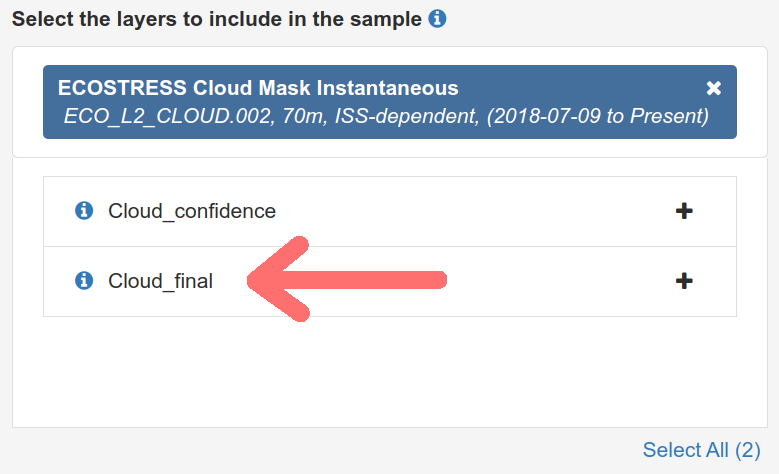
\includegraphics[width=\columnwidth]{Cloud_final.png}
			\end{center}
			\begin{itemize}[leftmargin=*]
				\item Simple \& straightforward.
				\item Pixels with values = 0 have been determined by the algorithm as ``not cloudy''.
				\item Pixels with values = 1 have been determined by the algorithm as ``cloudy''.
				\item Includes QA Stats for confidence in cloudiness determination, 0 = ``confidently clear'', 1 = ``probably clear'', and 2 =``probably cloudy'', and 3 = ``confidently cloudy''.
				\item Easy to visualize clouds in QGIS.
				\item Only available from late 2022 on!
			\end{itemize}
		\end{tcolorbox}
		\begin{tcolorbox}[colback=yellow!5!white,colframe=IceCreamLeaf, colbacktitle=IceCreamLeaf,title=SDS\_CloudMask]
			\begin{center}
				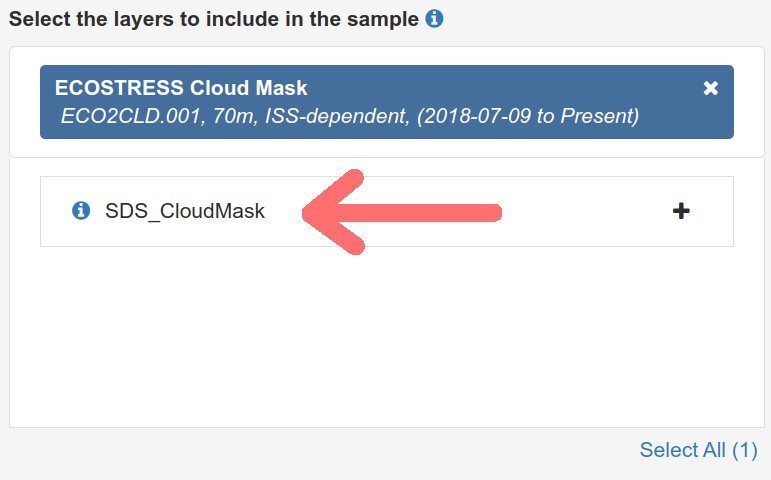
\includegraphics[width=\columnwidth]{SDS_CloudMask.png}
			\end{center}
			\begin{itemize}[leftmargin=*]
				\item Previous version of \textit{Cloud\_final}.
				\item Not as user-friendly.
				\item Best to visualize through A$\rho\rho$EEARS built-in graphs.
				\item Contains cloud information in addition to the tests used to determine cloudiness.
			\end{itemize}
		\end{tcolorbox}
		\begin{tcolorbox}[colback=yellow!5!white,colframe=IceCreamLeaf,
			colbacktitle=IceCreamLeaf,title=SDS\_QC]
			\begin{center}
				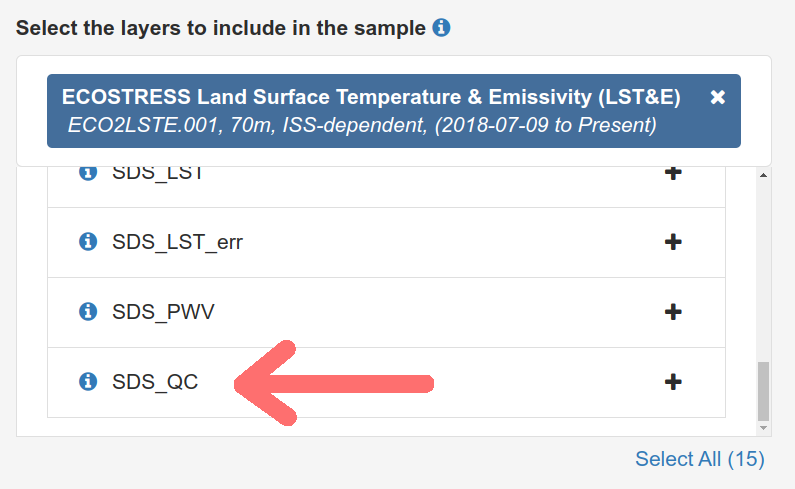
\includegraphics[width=\columnwidth]{SDS_QC.png}
			\end{center}
			\begin{itemize}[leftmargin=*]
				\item Broad quality control.
				\item Not as user-friendly.
				\item Best to visualize through A$\rho\rho$EEARS built-in graphs.
				\item Contains cloud information in addition to other quality metrics regarding missing pixels and atmosphere conditions.
			\end{itemize}
		\end{tcolorbox}
	\end{tcbraster}
	
	\vspace{.25em}
	
	\hrule
	
	\vspace*{.75em}
	
	To showcase the differences in these layers, let's create a new request in A$\rho\rho$EEARS for our new Vancouver Island shapefile for the week between Christmas Eve 2022 and New Year's Day 2023.
	
	24. Head over to \href{https://appeears.earthdatacloud.nasa.gov/}{https://appeears.earthdatacloud.nasa.gov/} and sign in.
	
	25. Click the \textit{Extract} dropdown menu to select Area. Next select Start a New Request.
	
	26. Use the screenshot below to set up your request. Name your sample, upload your Vancouver Island \textit{.zip} shapefile, enter \textit{12-24-2022} and \textit{01-01-2023} as start and end dates, and select ECOSTRESS land surface temperature (\textit{SDS\_LST}), \textit{SDS\_QC}, \textit{Cloud\_final}, and \textit{SDS\_CloudMask} as layers. Keep GeoTiff as the format and select \textit{Native Projection} for the projection. Click \textit{Submit}.
	
	\centerline{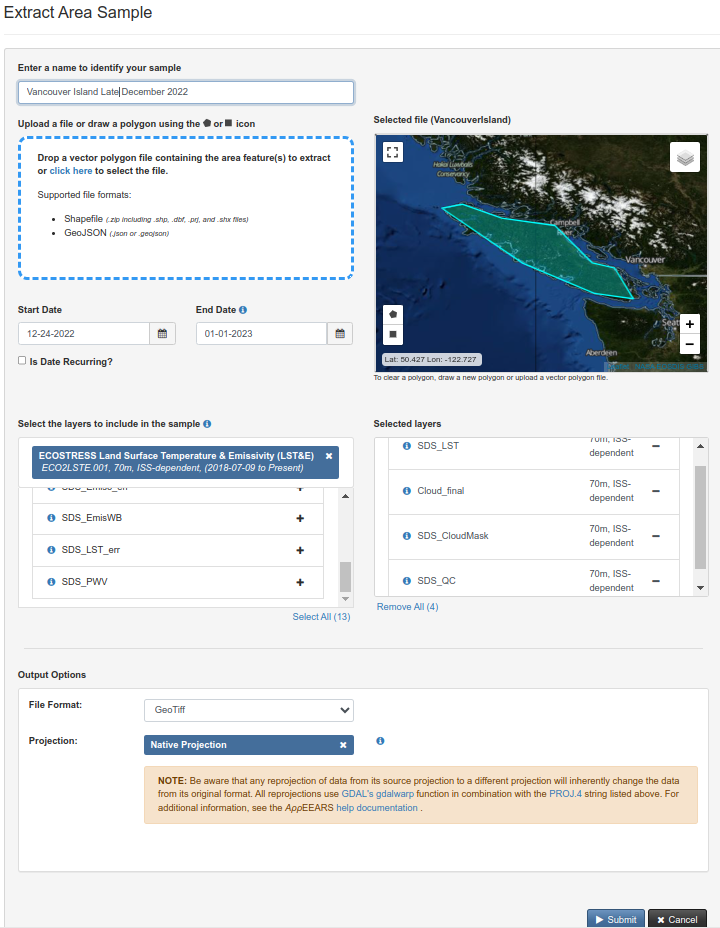
\includegraphics[width=.75\textwidth]{ExtractVancouver.png}}
	
	27. Use the \textit{Explore} dropdown menu to track the status of your request. 
	
	\vspace{.25em}
	
	\centerline{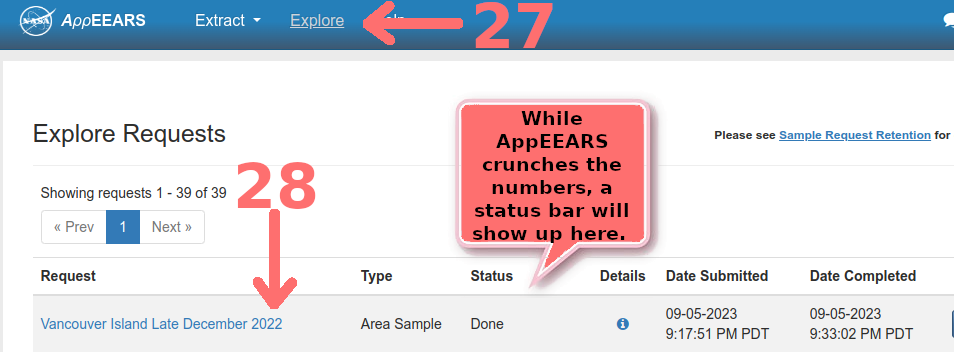
\includegraphics[width=.75\textwidth]{ExploreRequest.png}}
	
	28. When the request is complete, click on the name of your request to access the layer stats.
	
	29. In the meantime, let's visualize some of the cloud data. I have already accessed the \textit{Cloud\_final} layer for Vancouver Island from 1/1/2023. 
	
	\begin{tcolorbox}[colback=yellow!5!white,title=\textbf{Vancouver Island \textit{Cloud\_final} Layer Files}]
			
		\textbf{Please download these three GeoTIFF files, saving them somewhere logical and accessible, such as the same folder you used for the Vancouver Island shapefile:}
			
		\vspace{-1em}
			
		\begin{itemize}
			\item \href{https://jeremydforsythe.github.io/icecream-tutorials/Tutorial4_TemperatureCompetition/ECO_L2_CLOUD.002_Cloud_final_doy2023001105856_aid0001.tif}{ECO\_L2\_CLOUD.002\_Cloud\_final\_doy2023001105856\_aid0001.tif}
			\item \href{https://jeremydforsythe.github.io/icecream-tutorials/Tutorial4_TemperatureCompetition/ECO_L2_CLOUD.002_Cloud_final_doy2023001123515_aid0001.tif}{ECO\_L2\_CLOUD.002\_Cloud\_final\_doy2023001123515\_aid0001.tif}
			\item \href{https://jeremydforsythe.github.io/icecream-tutorials/Tutorial4_TemperatureCompetition/ECO_L2_CLOUD.002_Cloud_final_doy2023001141155_aid0001.tif}{ECO\_L2\_CLOUD.002\_Cloud\_final\_doy2023001141155\_aid0001.tif}
		\end{itemize}
			
	\end{tcolorbox}
	
	30. Switch over to QGIS, where you should still have your shapefile loaded as a layer. Load these three GeoTIFFs into active layers by double clicking on each in the browser window.
	
	\centerline{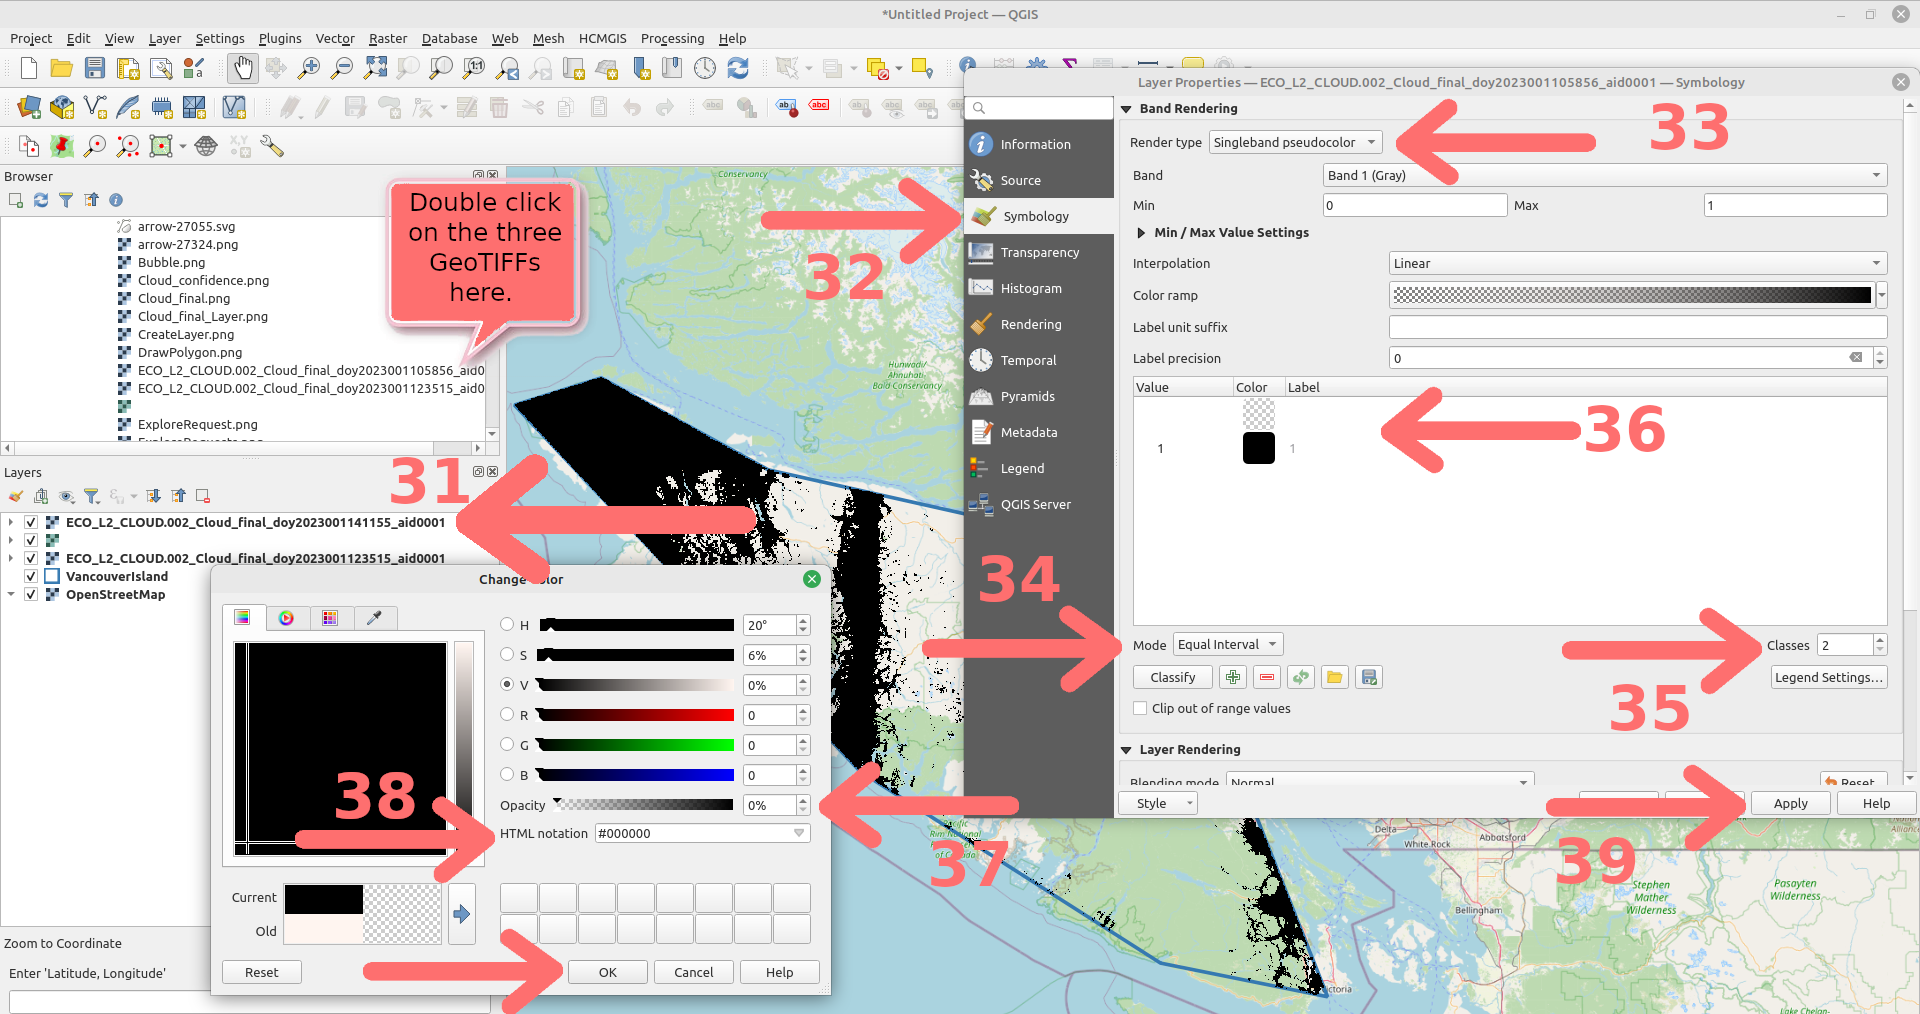
\includegraphics[width=.875\textwidth]{Cloud_final_AddLayer.png}}
	
	31. Right click on one of the layers in the \textit{Layer} browser, and select \textit{Properties}.
	
	32. In the panel, make sure \textit{Symbology} is selected.
	
	33. Change \textit{Render type} to \textit{Singleband pseudocolor}, which tells QGIS that we want this layer to be in color.
	
	34. Change \textit{Mode} to \textit{Equal Interval}. Now, we have told QGIS that we want this layer to be to have different colors for each value. 
	
	35. Change \textit{Classes} to \textit{2}. Remember Cloud\_final has only two values. 0 = ``not cloudy'' and 1 = ``cloudy''. Now we can change the color for each value.
	
	36. Right click on Windows/Linux or ctrl-click on Mac for the first value, 0. 
	
	37. Since 0 = ``not cloudy'', lets change this to be completely transparent by sliding the \textit{Opacity} bar all the way to zero. Click \textit{OK} and then right click on Windows/Linux or ctrl-click on Mac for the second value, 1. 
	
	38. If you are feeling particularly dark, make the clouds black by typing ``\#000000'' in the HTML notation box (this is HTML code for black.) Click \textit{OK}.
	
	39. Click \textit{Apply} to apply the color changes to your map.
	
	40. Repeat these steps for the other two Cloud\_final layers. You now have a cloudiness map for New Year's Day 2023 on Vancouver Island.
	
	41. Checking back on our Vancouver Island request in A$\rho\rho$EEARS. If it is ready, you can browse through the different layers shows to see how the quality and cloud metrics work. 
	
	\textbf{Cloud\_final:}
	
	\centerline{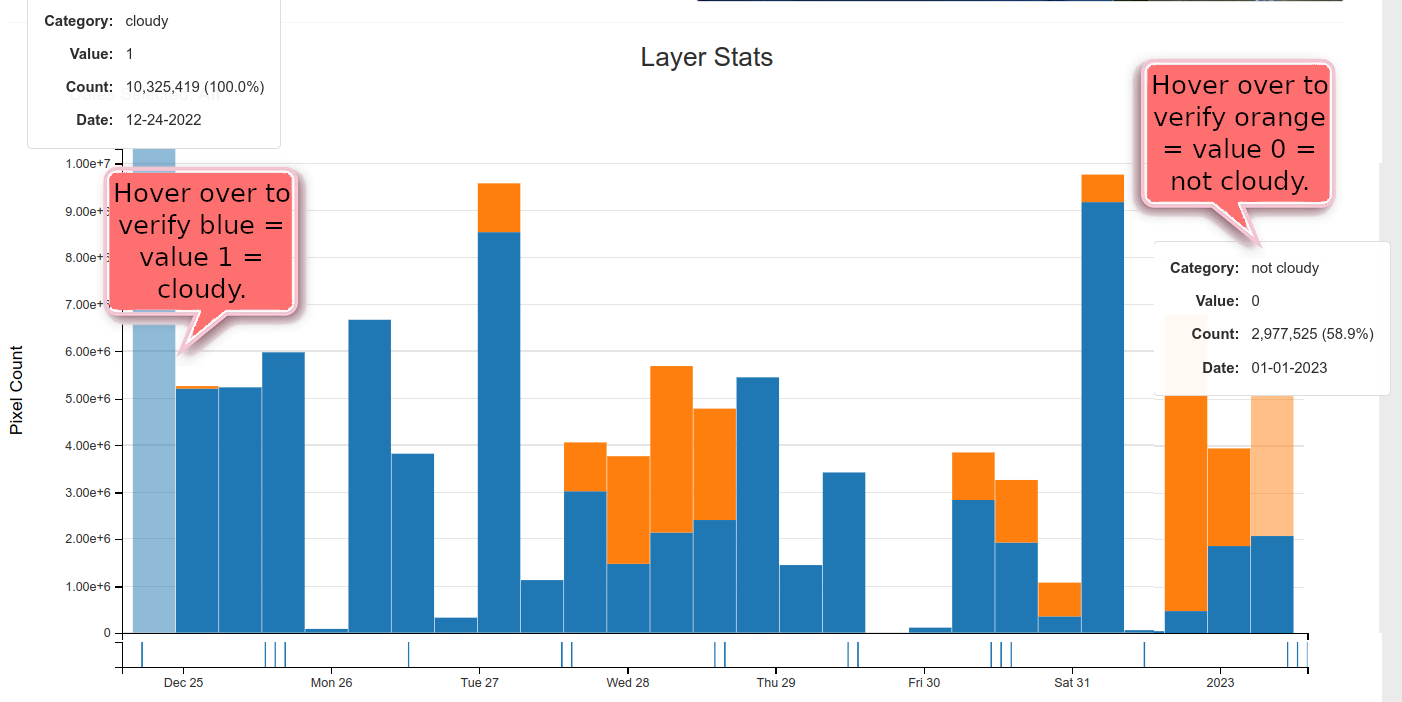
\includegraphics[width=.85\textwidth]{Cloud_final_Layer.png}}
	
	\textbf{Cloud\_confidence:}
	\centerline{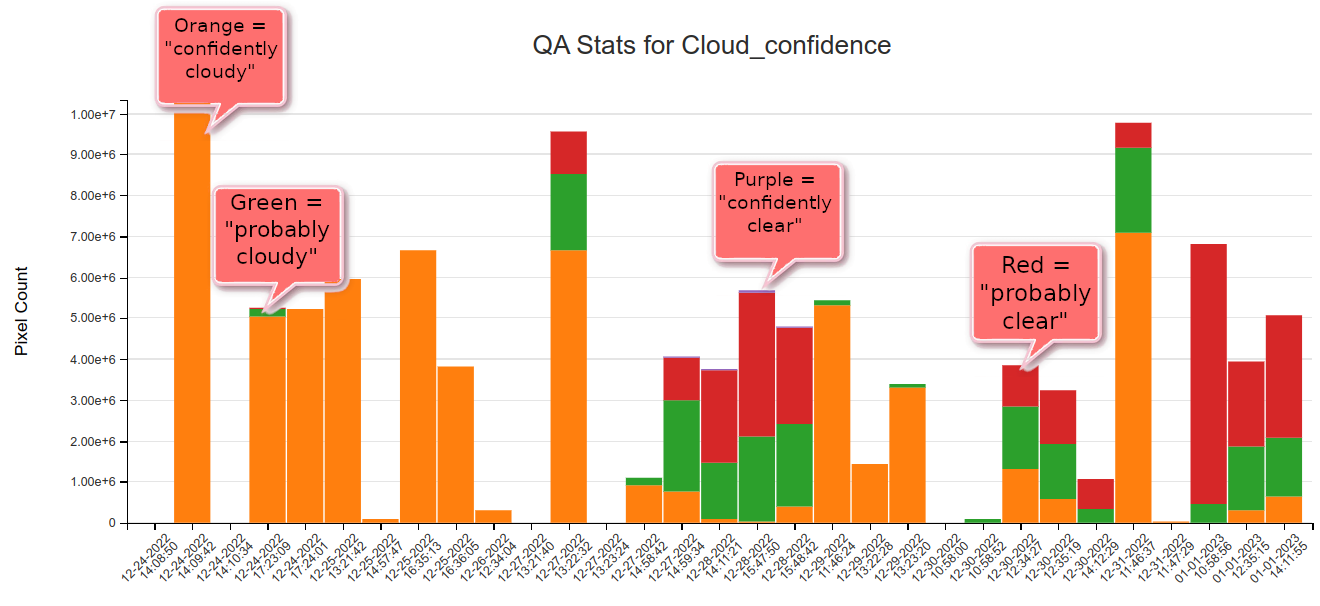
\includegraphics[width=.85\textwidth]{Cloud_confidence.png}}
	
	\textbf{SDS\_CloudMask:}
	\centerline{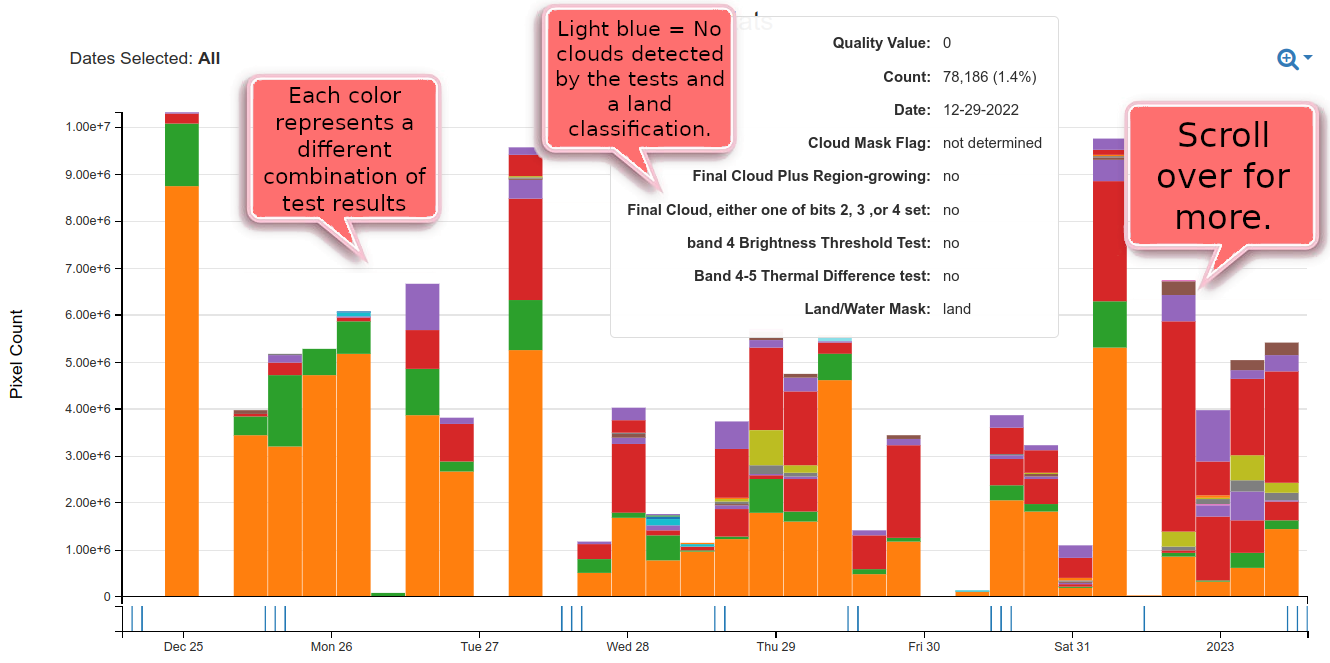
\includegraphics[width=.85\textwidth]{SDS_CloudMask_Layer.png}}
	
	\clearpage
	
	\textbf{SDS\_QC:}
	\centerline{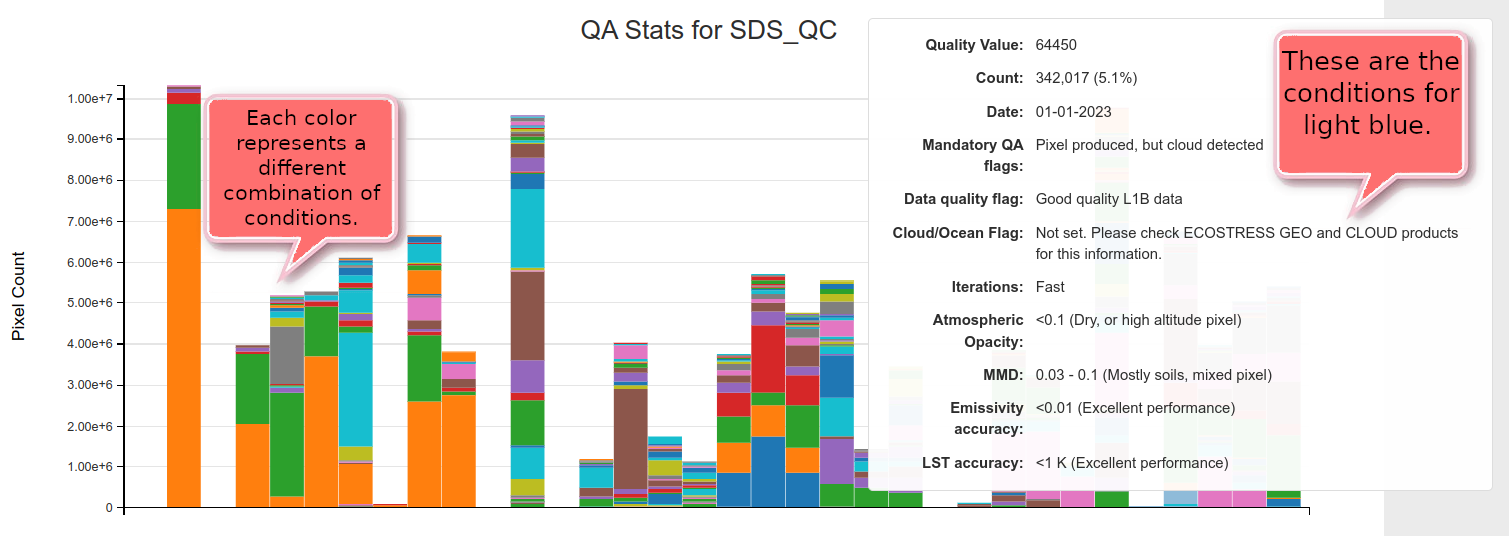
\includegraphics[width=\textwidth]{SDS_QC_Layer.png}}
	
	\vspace{.5em}
	
	The layers we have described here start simple and increase in complexity. As a general rule, we suggest using the simplest tools to complete your task. So, if your desired data is after November 2022, stick with the Cloud\_final layer. If it is before November 2022, use the SDS\_CloudMask. Finally, as your interest in remote sensing grows, you can learn more about the SDS\_QC layer in the \href{https://lpdaac.usgs.gov/documents/423/ECO2_User_Guide_V1.pdf}{ECOSTRESS Level 2 Product User Guide.}
	
	\section{Temperature Competition}
	
	By the end of the next tutorial, you will have all of the skills to generate a map showcasing the highest and lowest temperatures for your hometown. For now, let's focus on acquiring the data.
	
	\begin{tcolorbox}[colback=yellow!5!white,colframe=IceCreamLeaf,title=\textbf{Temperature Competition Instructions}]
		\begin{enumerate}
			\item Start a new project and create a shapefile for your hometown, favorite place you have lived, or somewhere you wish to move in the future using the steps outlined in this tutorial.
			\item  Use the same procedure we followed in \href{https://jeremydforsythe.github.io/icecream-tutorials/Tutorial2_AccessingRemoteSensingDataWithAppears/Tutorial2_AccessingRemoteSensingDataWithAppears.pdf}{Tutorial \#2 Accessing Remote Sensing Data With A$\rho\rho$EEARS} to create a new request in A$\rho\rho$EEARS, using your hometown shapefile, to access ECOSTRESS land surface temperature (SDS\_LST) and cloud data (Cloud\_final \& SDS\_CloudMask)  for the entire last calendar year. (This may take several hours).
			\item On your own time, determine which passes have the hottest and coldest observations of land surface temperature during the last calendar year and download those GeoTIFF data files somewhere you can access. We will use them in a future tutorial to finish the competition. This is a similar process to our Death Valley temperature in \href{https://jeremydforsythe.github.io/icecream-tutorials/Tutorial2_AccessingRemoteSensingDataWithAppears/Tutorial2_AccessingRemoteSensingDataWithAppears.pdf}{Tutorial \#2 Accessing Remote Sensing Data With A$\rho\rho$EEARS}.  
		\end{enumerate}
		
		\kulbox{\textbf{NOTE:} It is possible that if you selected a very large geographic area for your shapefile that the filesize with exceed the A$\rho\rho$EEARS file size limit. If this is the case, you could consider selecting a smaller area or submitting multiple requests, one for each layer.}
		
	\end{tcolorbox} 

	You can ask your classmates for suggestions if you get stuck, but remember to complete the work on your own. You will need these skills for future projects!

	\centerline{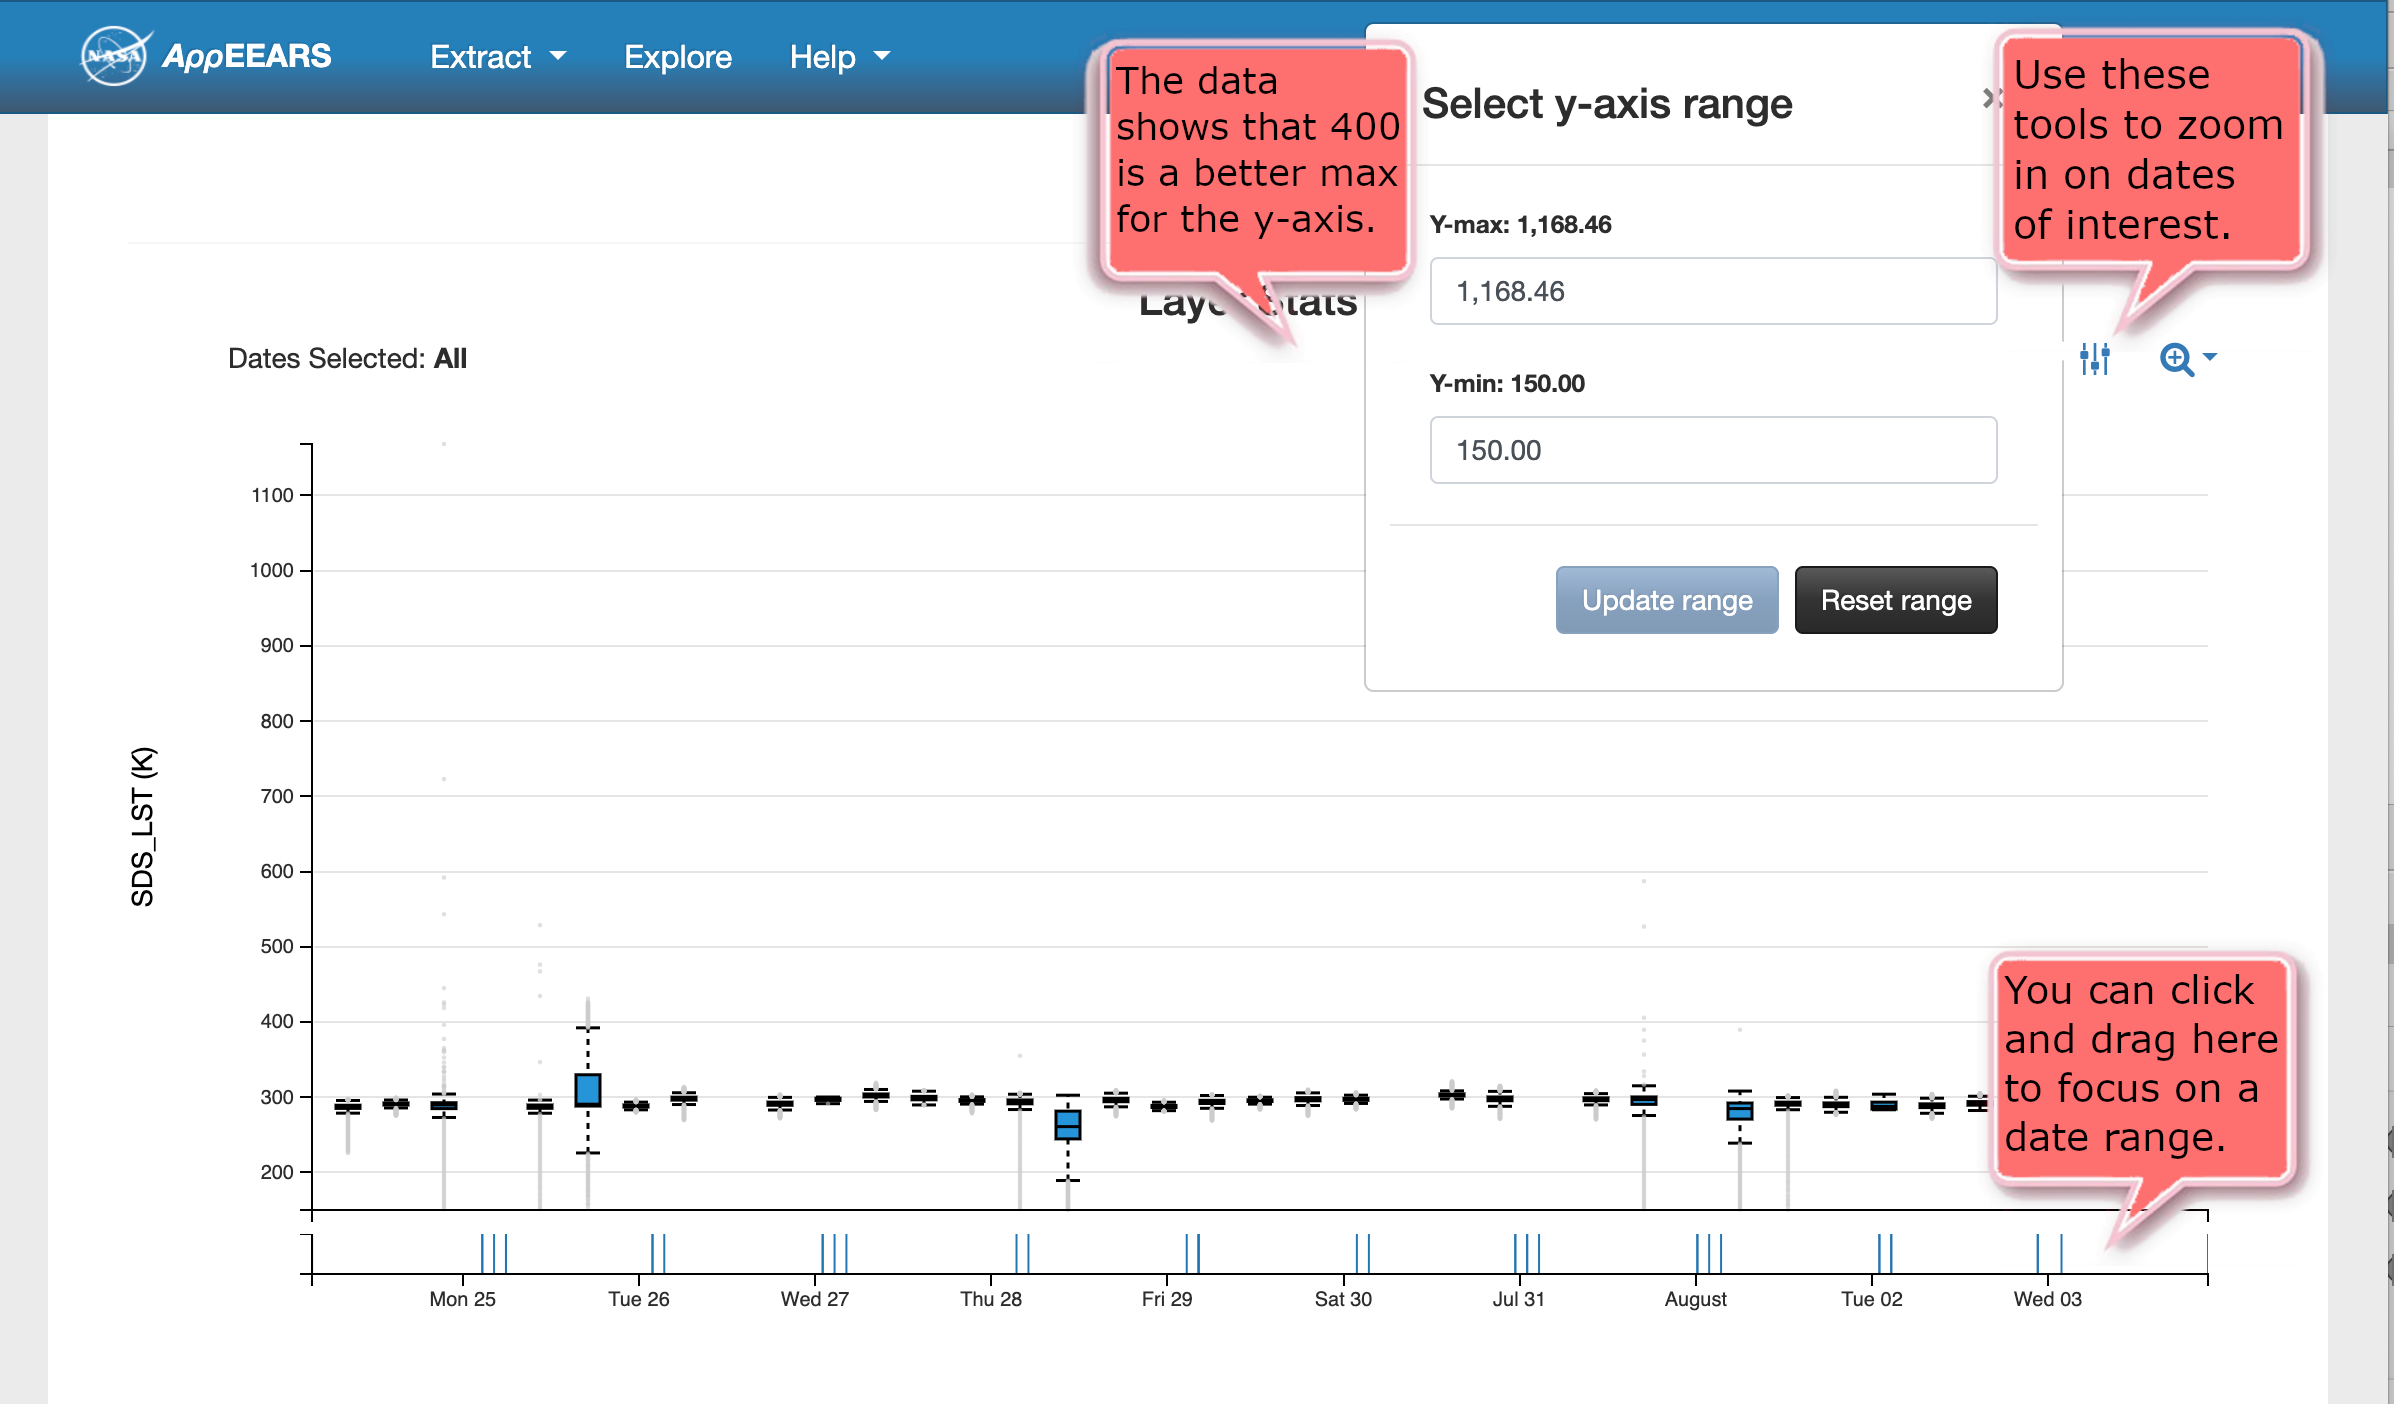
\includegraphics[width=\textwidth]{AppeearsZoom.png}}

	\kulbox{\textbf{NOTE:} The A$\rho\rho$EEARS graphing interface can be customized with options to zoom in on certain ranges of dates (x-axis) and values (y-axis). For instance, I find that I need to change the defaults in order to see the daily changes in temperatures clearly. You may also need to do this to select which days have the hottest and coldest temperatures. See screen shot above.}

	\kulbox{\textbf{NOTE:} It is entirely possible for ECOSTRESS to produce bad data with extreme and unrealistic values for land surface temperature. Make sure you are filtering for clouds. Also, keep in mind that the typical range for surface temperatures varies between -15 $^\circ$F to 115 $^\circ$F. \href{https://doi.org/10.1029/2018GL078133}{Antartica once witnessed frigid temperatures around -145 $^\circ$F} and the \href{https://jeremydforsythe.github.io/icecream-tutorials-main/Tutorial5_AddingElementsToMaps/Extreme Maximum Land Surface Temperatures.pdf} {theoretical maximum possible ground surface temperature has been estimated to be 212 $^\circ$F.} It is unlikely you will find good quality obversations near those extremes for your hometown.}
	
	\begin{tcolorbox}[colback=yellow!5!white,colframe=IceCreamLeaf,title=\textbf{Next Tutorial}]
		Next time you will learn how to make professional maps in QGIS and pull all of your new skills together to make a map with this new data for your hometown that showcases the highest and lowest temperatures for the last calendar year. 
	\end{tcolorbox}

	%%%%%%%%%%%%%%%%%%%%%%%%%%%%%%%%%%%%%%%%%%%%%%%%%%%%%%%%%%%%%%%%%%%%%%%%%%%%%%%%%%% Begin End Matter
	
	\vspace{.25em}
	
	\hrule
	
	\vspace{1 em}
	
	\begin{tcolorbox}[colback=yellow!5!white,colframe=IceCreamOrbit,title= \vspace{.2em} \Large Map of the Week Assignments]
		\addcontentsline{toc}{section}{Map of the Week Assignments}
		\large
		\begin{enumerate}
			\item Read about how your choice of colors in maps can be very important in the article: \href{https://theconversation.com/how-rainbow-colour-maps-can-distort-data-and-be-misleading-167159}{How rainbow colour maps can distort data and be misleading.}
			\item Submit the map of your hometown, like the timezone map we made in \href{https://jeremydforsythe.github.io/icecream-tutorials/Tutorial3_MakingBasicMapsInQGIS/Tutorial3_MakingBasicMapsInQGIS.pdf}{Tutorial \#3 Making Basic Maps In QGIS}, with your favorite basemap (Google Satellite, ESRI Imagery, ESRI Delorme, etc,). Make sure it includes an outline of your hometown created with your new shapefile you made today. We'll add the temperature data in the future.  
			\item Include a few sentences describing how you choose the borders of your shapefile and your design choices of your map. 
			\item Save GeoTIFF files to your computer of the hottest and coldest land surface temperature observations for your hometown last calendar year. Bring them for the next tutorial, you don't need to submit these to Canvas.
		\end{enumerate}
		
		Submit your map via Canvas before Monday's class.
	\end{tcolorbox}
	
	\vfill
	
	\hrule
	
	\vspace{1em}
	
	\textbf{Recommended Citation:} Forsythe, J.D., G.R. Goldsmith, and J.B. Fisher. 2023. Observing Earth from Above Tutorials. Chapman University. \url{https://jeremydforsythe.github.io/icecream-tutorials/}
	
	\vspace{1em}
	
	This work is supported by funding from NASA ECOSTRESS Mission Grant \#80NSSC23K0309 (I.C.E. C.R.E.A.M.: Integrating Communication of ECOSTRESS Into Community Research, Education, Applications, and Media).
	
\end{document}
